%----------------------------------------------------------------------------------------
%	PACKAGES AND OTHER DOCUMENT CONFIGURATIONS
%----------------------------------------------------------------------------------------

\documentclass[11pt, a4paper, oneside]{Thesis} % Paper size, default font size and one-sided paper
\usepackage[cm-default]{fontspec}
%\graphicspath{{Pictures/}} % Specifies the directory where pictures are stored
\usepackage{amssymb,amsmath}

% package to activate greek language - the sequence languages appear below is IMPORTANT!!!
%\usepackage[greek,english]{babel}
%\usepackage{xunicode}
\usepackage{xltxtra}

\usepackage{xgreek}   % Ελληνικό Hyphenation, αφαιρέστε το αν δεν έχετε εγκατεστημένο το xgreek
\usepackage{varioref}

%\usepackage{etoolbox}% http://ctan.org/pkg/etoolbox
\setlength{\parindent}{15pt}


% FONTS
%\usepackage{xunicode}    %  KANONIKA TO XRHAZESAI GIA TA ELLHNIKA - ALLA YPERKALYPTETE APO TO xltxtra
\usepackage{xcolor}
\defaultfontfeatures{Mapping=tex-text} % converts LaTeX specials (``quotes'' --- dashes etc.) to unicode
 %\setromanfont [Ligatures={Common}, BoldFont={GFS Artemisia Bold}, ItalicFont={Gentium Italic}]{Gentium}
%\setmonofont[Scale=0.8]{Monaco} 
\setmainfont[Mapping=tex-text]{DejaVu Sans}

\usepackage[square, numbers, comma, sort&compress]{natbib} % Use the natbib reference package - read up on this to edit the reference style; if you want text (e.g. Smith et al., 2012) for the in-text references (instead of numbers), remove 'numbers' 
\hypersetup{linkcolor=black, urlcolor=black, colorlinks=true} % Colors hyperlinks in blue - change to black if annoying
\title{\ttitle} % Defines the thesis title - don't touch this

\usepackage{listings}             % Include the listings-package
\lstset{language=Java}          % Set your language (you can change the language for each code-block optionally)

\begin{document}

\frontmatter % Use roman page numbering style (i, ii, iii, iv...) for the pre-content pages

\setstretch{1.3} % Line spacing of 1.3

% Define the page headers using the FancyHdr package and set up for one-sided printing
\fancyhead{} % Clears all page headers and footers
\rhead{\thepage} % Sets the right side header to show the page number
\lhead{} % Clears the left side page header

\pagestyle{fancy} % Finally, use the "fancy" page style to implement the FancyHdr headers

\newcommand{\HRule}{\rule{\linewidth}{0.5mm}} % New command to make the lines in the title page

% PDF meta-data
\hypersetup{pdftitle={\ttitle}}
\hypersetup{pdfsubject=\subjectname}
\hypersetup{pdfauthor=\authornames}
\hypersetup{pdfkeywords=\keywordnames}

%----------------------------------------------------------------------------------------
%	TITLE PAGE
%----------------------------------------------------------------------------------------

\begin{titlepage}

\begin{center}

 \begin{minipage}{0.6\textwidth}
\begin{flushright} 
  \textsc{\LARGE \univname}\\[0.5cm] % University name
  \textsc{\LARGE \deptname}\\[1.5cm] % University name
\end{flushright}
\end{minipage}
\begin{minipage}{0.3\textwidth}
\begin{flushright} 
 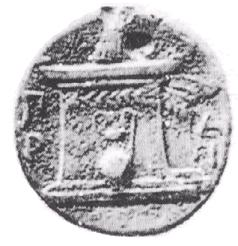
\includegraphics[scale=0.35]{Figures/logo.jpg}
\end{flushright}
\end{minipage}


\vspace*{50pt}
\textsc{\Large \degreename}\\[0.2cm] % Thesis type

\HRule \\[0.4cm] % Horizontal line
{\huge \bfseries \ttitle}\\[0.4cm] % Thesis title
\HRule \\[1.5cm] % Horizontal line
 
\begin{minipage}{0.4\textwidth}
\begin{flushleft} \large
\textbf{\LARGE
\href{https://github.com/arischmod/}{\authornames} % Author name - remove the \href bracket to remove the link
}
\end{flushleft}
\end{minipage}
\begin{minipage}{0.5\textwidth}
\begin{flushright} \large
\emph{Επιβλέπων Καθηγητης:} \\
\href{http://galaxy.hua.gr/~varlamis/index.php?cat=news}{\supname}\\[1.0cm] % Supervisor name - remove the \href bracket to remove the link  

\emph{Μέλη της \\Εξεταστικής Επιτροπής:}\\
Μιχαήλ Δημήτρης\\
Κωνσταντίνα Βασιλοπούλου
\end{flushright}
\end{minipage}\\[7cm]

%{\large \today}\\[4cm] % Date
%\includegraphics{Logo} % University/department logo - uncomment to place it

Αθήνα,\\ Φεβρουάριος 2014

\vfill
\end{center}

\end{titlepage}


%----------------------------------------------------------------------------------------
%	Περίληψη
%----------------------------------------------------------------------------------------
\label{perilipsi}
\addtotoc{Περίληψη} % Add the "Abstract" page entry to the Contents

\perilipsi{\addtocontents{toc}{} % Add a gap in the Contents, for aesthetics
\noindent
\textbf{\ttitle}\\

\noindent
Η παρούσα έρευνα περιλαμβάνει την μελέτη της θεωρίας και των μεθόδων που χρειάζονται για την δημιουργία ενός συστήματος συστάσεων το οποίο εκμεταλλεύεται τις 
πληροφορίες που αντλεί από ένα 
κοινωνικό γράφο. Επίσης περιγράφεται ο σχεδιασμός μιας πλατφόρμας εύρεσης κοινοτήτων χρηστών που θα χρησιμοποιηθεί ως εργαλείο για την επίτευξη των παραπάνω.\\
Αρχικά σε ένα πρώτο κομμάτι της έρευνας θα αναλυθούν οι βασικές έννοιες και προσεγγίσεις των Συστημάτων Συστάσεων σύμφωνα με την σχετική βιβλιογραφία.
Στην συνέχεια μελετάται πως ένα τέτοιο σύστημα μπορεί να βελτιωθεί χρησιμοποιώντας την επιστήμη των κοινωνικών δικτύων. 
Ακολουθεί η παρουσίαση της δικής μας υλοποίησης ενός τέτοιου συστήματος και τέλος περιγράφεται η ενσωμάτωση του προγράμματός μας σε ένα υπάρχον
σύστημα προσωποποίησης ώστε να επεκταθεί η λειτουργία του και να βελτιωθεί η ακρίβεια των αποτελεσμάτων του.\\[3.0cm] 

\noindent
\textbf{ΘΕΜΑΤΙΚΗ ΠΕΡΙΟΧΗ:} Συστήματα Συστάσεων βασιζόμενα σε Κοινωνικά Δίκτυα (SNRS)

\noindent
\textbf{ΛΕΞΕΙΣ ΚΛΕΙ∆ΙΑ:} Προσωποποίηση, Συστήματα Συστάσεων, Κοινωνικά Δίκτυα, Κοινοτικές 
Δομές Δικτύων, Εξόρυξη Δεδομένων από Κοινωνικούς Γράφους

}

\clearpage % Start a new page
%----------------------------------------------------------------------------------------
%	ABSTRACT PAGE
%----------------------------------------------------------------------------------------

\addtotoc{Abstract} % Add the "Abstract" page entry to the Contents
\abstract{\addtocontents{toc}{} % Add a gap in the Contents, for aesthetics
\noindent
\textbf{\ttitleen}\\

\noindent
This research includes the study of theory and methods needed to create a Recommender System 
which exploits the information derived from a social graph. 
Also we outline the design of a platform which locates User Communities that will be used as 
a tool for achieving the above.
The first part of the research analyzes the basic concepts and approaches of Recommender
Systems in accordance with the relevant literature.
Furthermore we make a study of how such a system can be improved if combined with the field of 
social networks.
Next is the presentation of our own implementation of such a system and finally we describe
the integration of our program in an existing
personalization system to extend function and improve the accuracy of its results. \\[3.0cm] 

\noindent
\textbf{SUBJECT AREA:} Social Network based Recommender System (SNRS)


\noindent
\textbf{KEYWORDS:} Personalization, Recommender Systems, Social Network, 
Community Structure in Networks, Mining Data from Social Graphs

}

\clearpage % Start a new page

%----------------------------------------------------------------------------------------
%	ACKNOWLEDGEMENTS
%----------------------------------------------------------------------------------------

\setstretch{1.3} % Reset the line-spacing to 1.3 for body text (if it has changed)

\acknowledgements{\addtocontents{toc}{\vspace{1em}} % Add a gap in the Contents, for aesthetics
\noindent
Η εκπόνηση της παρούσας πτυχιακής εργασίας ξεκίνησε στο Τμήμα Πληροφορικής και Τηλεματικής
του Χαροκοπείου Πανεπιστημίου Αθηνών τον Οκτώβριο του 2013 και ολοκληρώθηκε τον
Φεβρουάριο του 2014. Σε αυτό το σημείο, θα ήθελα να εκφράσω τις ευχαριστίες μου σε όλους
όσους συνέβαλαν άμεσα ή έμμεσα στην ολοκλήρωση της πτυχιακής εργασίας μου και γενικότερα
των προπτυχιακών σπουδών μου.

  Αρχικά θα ήθελα να εκφράσω ιδιαίτερες ευχαριστίες στον επιβλέποντα καθηγητή,
Ηρακλή Βαρλάμη, για την καθοδήγηση, την ενθάρρυνση 
αλλά και την εμπιστοσύνη που μου έδειξε αναθέτοντας μου την συγκεκριμένη εργασία.
  
  Στη συνέχεια, θα ήθελα να ευχαριστήσω την SciFy και τα μέλη της, ιδιαίτερα τον 
Βασίλη Σαλαπάτα και Γιωργο Γιαννακοπουλο των οποίων οι γνώσεις, οι συμβουλές και η στήριξη  
ήταν ζωτικής σημασίας για την ολοκλήρωση της πτυχιακής εργασίας. 
    
  Τέλος, ευχαριστώ το κοντινό οικογενειακό και φιλικό μου περιβάλλον,
Χρήστο, Ευγενία, Αγγελική, Morgan, Παύλο, Λουκά, Γιάννη, Ντούμα, Εβίτα,  
για την καθημερινή κατανόηση, ψυχολογική στήριξη και υπομονή.
}
\clearpage % Start a new page


%----------------------------------------------------------------------------------------
%	LIST OF CONTENTS PAGES
%----------------------------------------------------------------------------------------

\pagestyle{fancy} % The page style headers have been "empty" all this time, now use the "fancy" headers as defined before to bring them back

\lhead{\emph{Περιεχόμενα}} % Set the left side page header to "Contents"

\tableofcontents % Write out the Table of Contents

%\addtocontents{toc}{\vspace{2em}} % Add a gap in the Contents, for aesthetics

%----------------------------------------------------------------------------------------
%	THESIS CONTENT - CHAPTERS
%----------------------------------------------------------------------------------------

\mainmatter % Begin numeric (1,2,3...) page numbering

\pagestyle{fancy} % Return the page headers back to the "fancy" style


\chapter{Εισαγωγή} % Main chapter title

\label{Εισαγωγή} % Change X to a consecutive number; for referencing this chapter elsewhere, use \ref{ChapterX}

\lhead{Κεφάλαιο 1. \emph{Εισαγωγή}} % Change X to a consecutive number; this is for the header on each page - perhaps a shortened title
\noindent
Η συνεχόμενη αύξηση του μεγέθους και της χρήσης του διαδικτύου έχει ως επακόλουθο
οι υπηρεσίες να υπερφορτώνονται με πληροφορίες και η χρήση τους να γίνεται
όλο και πιο πολύπλοκη. Οι χρήστες καθημερινά καλούνται να αντιμετωπίσουν
την υπερπληροφόρηση η οποία συχνά μάλιστα τους εμποδίζει από το να εκπληρώσουν τον αρχικό τους σκοπό.
Επομένως γίνεται όλο και πιο επιτακτική η ανάγκη για \emph{προσωποποίηση των υπηρεσιών}.
Προσωποποίηση θεωρείται η δυνατότητα μιας υπηρεσίας να λαμβάνει υπόψιν τις προτιμήσεις του κάθε χρήστη 
κατά την διαμόρφωση του περιεχομένου της.

\section{Ανάλυση Του Προβλήματος}
\noindent
Η παρούσα εργασία ξεκινά με μια βασική υπόθεση: Έχουμε στη διάθεσή μας μια \emph{γενικευμένη μηχανή προσωποποίησης περιεχομένου} 
\setlanguage{english} \emph{(\hyperref[PServer]{PServer 3.5})} \setlanguage{greek}.
Πρόκειται για έναν \emph{εξυπηρετητή} ο οποίος όπως και κάθε μηχανή που προσφέρει
προσωποποίηση, λαμβάνει υπόψιν τις προτιμήσεις του κάθε χρήστη και 
ακολούθως διαμορφώνει το περιεχόμενό της σύμφωνα με τα 
χαρακτηριστικά του κάθε ενός.
Στην περίπτωση ενός δικτυακού τόπου ο PServer είναι ένας ακόμα \emph{εξυπηρετητής} 
ο οποίος αναλαμβάνει να προσωποποιήσει οποιαδήποτε υπάρχουσα υπηρεσία,
συλλέγοντας πληροφορίες για τους χρήστες και την αλληλεπίδραση τους με αυτήν και τελικά παρέχοντας τις πληροφορίες που χρειάζονται για την προσωποποίηση. 
Η διαδικασία αυτή για να πετύχει τους στόχους της εμπεριέχει ένα πλήρες \emph{Σύστημα Συστάσεων}. 
Για την λειτουργία του, διατηρεί προφίλ χρηστών τα οποία τροφοδοτεί με δημογραφικές πληροφορίες και πληροφορίες προτιμήσεων και στη συνέχεια μπορεί να προβλέψει: 
από όλο το εύρος των πιθανών προτιμήσεων ποιο είναι το υποσύνολο στο οποίο έγκειται ο κάθε χρήστης. 
Τελικώς, μπορεί να κάνει συστάσεις αντικειμένων στους χρήστες βασιζόμενος στην υπάρχουσα αλληλεπίδρασή τους με το σύστημα.

Καλούμαστε να επεκτείνουμε αυτό το σύστημα ώστε να δημιουργεί συστάσεις βασιζόμενο, όχι μόνο στις πληροφορίες των δημογραφικών στοιχείων και των προτιμήσεων, 
αλλά να μπορεί να προβλέπει την συμπεριφορά του κάθε χρήστη μελετώντας την κοινωνική δικτύωση των χρηστών της εφαρμογής. 
Με τον τρόπο αυτό αναμένουμε από το σύστημα να πριμοδοτεί περιεχόμενα με τα οποία είχαν
επαφή οι φίλοι κάποιου χρήστη έναντι περιεχομένων που έχουν δει μόνο άγνωστοι σε αυτόν χρήστες.
Για την εφαρμογή των παραπάνω, σχεδιάστηκε και υλοποιήθηκε ένα σύστημα (\textbf{socialPServer}) το οποίο επιτρέπει τον εντοπισμό των ενδιαφερόντων ενός 
χρήστη εξάγοντας συμπεράσματα από τα αντικείμενα 
τα οποία προτιμούν οι κοντινότεροι φίλοι του,
δοσμένου του κοινωνικού γράφου της εφαρμογής. 
Το σύστημα αυτό μπορεί να χαρακτηριστεί ως \textbf{Social Recommendation System}.

\section{Προσέγγιση}
\noindent
Τα \emph{κοινωνικά δίκτυα} από τη φύση τους αποτελούν πολύ σημαντική πηγή εξόρυξης δεδομένων, καθώς η δομή τους εμπεριέχει πληθώρα πληροφοριών για τα μελή τους.
Όταν μια εφαρμογή διατηρεί τον κοινωνικό γράφο των χρηστών της, μπορεί να εξάγει πληροφορίες οι οποίες ξεφεύγουν 
από τα πλαίσια της υπηρεσίας και αποκαλύπτουν στοιχεία για την πραγματική ζωή και συμπεριφορά των χρηστών. 
Αυτό προκύπτει από το γεγονός ότι ο άνθρωπος, ο οποίος από την φύση του είναι κοινωνικό όν, σε όλη την διάρκεια 
της ζωής του τείνει να ετεροκαθορίζεται και κατ' επέκταση να δρα επηρεασμένος από το κοινωνικό του περιβάλλον.
Έτσι ο τομέας του \emph{Social Analysis} αποκτά πολύ μεγάλη σημασία για την έρευνα αλλά και τις σημερινές ηλεκτρονικές υπηρεσίες.
Πλέον η εξαγωγή γνώσης δεν εξαρτάται μόνο από την αλληλεπίδραση του χρήστη με το σύστημα, αφού ο κάθε χρήστης δεν αντιμετωπίζεται σαν μονάδα αποκομμένος από το σύνολο 
αλλά σαν μέλος του. 
Η επίδραση που έχει η κοινότητα στο κάθε μέλος βεβαίως είναι αμφίδρομη διαδικασία αφού όπως ο κάθε χρήστης επηρεάζεται από το γύρο περιβάλλον του, έτσι και ολόκληρο το
κοινωνικό σύνολο διαμορφώνεται τελικά από τον κάθε ένα αυτόνομο χρήστη.

Για την πραγματοποίηση των παραπάνω, οι χρήστες της εφαρμογής ομαδοποιούνται σε κοινότητες χρηστών των οποίων τα μέλη έχουν μεταξύ τους ισχυρούς δεσμούς φιλίας. 
Έτσι σε επόμενο χρόνο μπορούν να σκιαγραφηθούν οι προτιμήσεις του κάθε χρήστη μέσω της ανάλυσης των συμπεριφορών και των προτιμήσεων των μελών της κοινότητας στην οποία ανήκει. 
Μέσω αυτής της διαδικασίας ο pServer θα είναι πλέον σε θέση να κάνει συστάσεις σε κάποιο χρήστη βασιζόμενος στις προτιμήσεις των κοντινότερων φίλων του
από τους οποίους, όπως και στην πραγματική ζωή, εκτιμάται ότι δέχεται και την υψηλότερη επιρροή.

 % Εισαγωγή

\chapter{Θεωρητική Ανάλυση και Αλγόριθμοι} % Main chapter title

\label{Θεωριτική Ανάληση} % Change X to a consecutive number; for referencing this chapter elsewhere, use \ref{ChapterX}

\lhead{Κεφάλαιο 2. \emph{Θεωρητική Ανάλυση}} % Change X to a consecutive number; this is for the header on each page - perhaps a shortened title


%----------------------------------------------------------------------------------------
%	SECTION 1
%----------------------------------------------------------------------------------------


\section{Προσωποποίηση}
\noindent
Η βασική φιλοσοφία ενός συστήματος Προσωποποίησης είναι \emph{να παρέχει στους χρήστες
τις πληροφορίες που θέλουν ή χρειάζονται, χωρίς να περιμένει να του ζητηθεί ρητά}.\cite{mulvenna2000personalization}\\
Τα δομικά στοιχεία της προσωποποίησης των δικτύων είναι:\\
- Η κατηγοριοποίηση και προεπεξεργασία των δεδομένων.\\
- H εξόρυξη των συσχετίσεων μεταξύ διαφορετικών ειδών δεδομένων.\\
- Ο προσδιορισμός των ενεργειών που θα προταθούν από το σύστημα.\cite{mobasher2000automatic}\\
Ο πιο διαδεδομένος τρόπος επίτευξης της προσωποποίησης είναι με την εφαρμογή ενός Συστήματος Συστάσεων. 
\cite{eirinaki2003web}



\section{Συστήματα Συστάσεων}
\noindent
Ένα \emph{Σύστημα Συστάσεων (Recommender System)} είναι ουσιαστικά ένας μηχανισμός που
ως πρώτο σκοπό έχει το να προβλέψει το ενδιαφέρον ενός χρήστη για αντικείμενα με τα 
οποία δεν έχει ακόμα επαφή.
Εντοπίζοντας και εμφανίζοντας στο χρήστη αντικείμενα με μέγιστο εκτιμώμενο ενδιαφέρον,
επιτυγχάνεται η προσωποποίηση μιας Web υπηρεσίας και ο χρήστης καταφέρνει να αποφύγει την υπερπληροφόρηση έχοντας πρόσβαση σε ένα υποσύνολο των αντικειμένων
της υπηρεσίας το οποίο τον ενδιαφέρει περισσότερο σύμφωνα με τις μέχρι στιγμής προτιμήσεις του.
Σε αυτήν την παράγραφο θα επιχειρήσουμε μία εισαγωγή στα Recommender Systems (συστήματα συστάσεων) και στις υπάρχουσες θεωρητικές και πρακτικές κατευθύνσεις. 
  
\subsection{Εισαγωγή Στα Συστήματα Συστάσεων}
\noindent
Στη μελέτη επισκόπησης των \emph{Adomavicius} και \setlanguage{english}  \emph{Tuzhilin} \cite{NGRS} \setlanguage{greek} όπου πραγματοποιήθηκε έρευνα σχετικά με το υπάρχον στάδιο 
των \setlanguage{english} Recommender systems, \setlanguage{greek} αντλήθηκαν και παρουσιάζονται τα παρακάτω στοιχεία.
  
Τα συστήματα συστάσεων αναδύθηκαν σαν ερευνητικό πεδίο μετά την εμφάνιση των πρώτων papers σχετικών με το collaborative filtering στα μέσα της δεκαετίας του 90. 
Τόσο στην ακαδημαϊκή κοινότητα αλλά και στον επιχειρηματικό κόσμο, την τελευταία δεκαετία, γίνονται προσπάθειες εύρεση και υλοποίηση νέων προσεγγίσεων. 
Το ενδιαφέρον παραμένει ακόμα υψηλό καθώς υπάρχουν πολλά ακόμα προβλήματα προς επίλυση και χώρος για την ανάπτυξη προσωποποιημένων εφαρμογών, καθώς οι χρήστες των διαδικτυακών
υπηρεσιών καλούνται να αντιμετωπίσουν την ολοένα και μεγαλύτερη υπερπληροφόρηση.

Σχετικές έννοιες είχαν ήδη αναφερθεί σε διαφορετικούς τομείς όπως στην ανάκτηση 
πληροφορίας \setlanguage{english}(information retrieval)\setlanguage{greek} 
αλλά και στο μάρκετινγκ,
αποτέλεσε όμως ανεξάρτητο πεδίο από την στιγμή που οι ερευνητές άρχισαν να μελετούν 
\emph{προβλήματα βαθμονόμησης \setlanguage{english} (ranking problems)}\setlanguage{greek} 
των συστάσεων. 
Ο πυρήνας ενός Συστήματος Συστάσεων είναι ουσιαστικά μια διαδικασία πρόβλεψης
αξιολογήσεων(rating) των αντικειμένων με τα οποία ο χρήστης δεν είχε ακόμα επαφή,
και στη συνέχεια βαθμονόμησης των αντικειμένων με βάση την αξιολόγηση,
ώστε τελικά να προταθούν στον χρήστη τα αντικείμενα με την υψηλότερη εκτιμώμενη αξιολόγηση.\\

Αν επιχειρήσουμε μια πιο τυπική διατύπωση των παραπάνω έχουμε:\\
Ένα σύνολο χρηστών $C$ και ένα σύνολο αντικειμένων $S$. \\
Επίσης έχουμε $u$ τη συνάρτηση χρησιμότητας ενός αντικειμένου $s$ για τον χρήστη $c$.
Τότε για τη συνάρτηση χρησιμότητας $u$ ισχύει ότι 

$u:C$x$S \rightarrow R$,  με R να είναι ένα καθορισμένο σύνολο (π.χ. μη αρνητικοί ακέραιοι ή πραγματικοί αριθμοί κάποιου εύρους).

Στην συνέχεια για κάθε χρήστη $c\in C$, θέλουμε να επιλέξουμε κάποιο αντικείμενο $\acute{s}\in S$ το οποίο να μεγιστοποιεί 
το εκτιμώμενο ενδιαφέρον (\emph{χρησιμότητα}) του χρήστη για αυτό.

Επομένως:   $\forall c\in C,  \acute{s_c}=\arg_{s\in S} \max u(c,s) $   

Συνήθως στα συστήματα συστάσεων η χρησιμότητα ενός αντικειμένου εκφράζεται με μια αξιολόγηση, εναλλακτικά η χρησιμότητα μπορεί να προκύπτει από μια καθορισμένη συνάρτηση κέρδους.
Ανάλογα με την φύση της εφαρμογής, η χρησιμότητα $u$ μπορεί είτε να δηλωθεί από τον χρήστη με την μορφή αξιολόγησης,
είτε να υπολογιστεί από την ίδια την εφαρμογή όπως στην περίπτωση της συνάρτησης κέρδους.

Κάθε μέλος του συνόλου χρηστών $C$ περιγράφεται από ένα \emph{προφίλ (userProfile)} που περιλαμβάνει προσωπικές πληροφορίες, όπως δημογραφικά στοιχεία ή προτιμήσεις.
Στην πιο απλή περίπτωση μοναδικό στοιχείο που χρειάζεται είναι ένα userID. 
Παρομοίως κάθε στοιχείο του συνόλου των αντικειμένων $S$ μπορεί να περιγράφεται από ένα σύνολο χαρακτηριστικών. 
\cite{NGRS}

\subsection{Μέθοδοι Συστάσεων}
\noindent
Hill, Resnick και Shardanand είναι μερικοί από τους θεμελιωτές 
της σύνθεσης κοινώς αποδεκτών μεθόδων για την παραγωγή συστάσεων.
\cite{hill1995recommending} \cite{resnick1994grouplens} \cite{shardanand1995social}\\
Έκτοτε το πρόβλημα έλαβε τις υπάρχουσες διαστάσεις του και άρχισε να μελετάται περαιτέρω.
  
Τα Συστήματα Συστάσεων υπάγονται στις ακόλουθες γενικές κατηγορίες ανάλογα με τον τρόπο προσέγγισης των αξιολογήσεων:

\begin{description}
\item \textbf{Content-based recommendations}  \hfill \\
Η πρόβλεψη των αξιολογήσεων προκύπτει από τις αξιολογήσεις που έχει κάνει ο χρήσης σε άλλα αντικείμενα. 
Επομένως τελικά προτείνονται αντικείμενα παρόμοια με αυτά που έχει αξιολογήσει θετικά στο παρελθόν.
\item \textbf{Collaborative recommendations}  \hfill \\
Η πρόβλεψη των αξιολογήσεων προκύπτει από τις αξιολογήσεις που έχουν κάνει άλλοι χρήστες της εφαρμογής, των οποίων τα προφίλ μοιάζουν με το προφίλ του χρήστη. 
Επομένως τελικά προτείνονται αντικείμενα τα οποία έχουν προτιμηθεί στο παρελθόν από χρήστες με κοινές προτιμήσεις ή χαρακτηριστικά.
\item \textbf{Hybrid approaches}  \hfill \\
Συνδυασμός των δυο παραπάνω μεθόδων.
\end{description} 

Σε όλες τις περιπτώσεις όταν τα άγνωστα ratings έχουν πλέον υπολογιστεί συνίστανται στον χρήστη τα αντικείμενα με την υψηλότερη προβλεπόμενη αξιολόγηση.
 
Στα πλαίσια αυτής της πτυχιακής επιθυμούμε να εξάγουμε συμπεράσματα εκμεταλλευόμενοι τις προτιμήσεις άλλων χρηστών δηλαδή 
να δημιουργήσουμε συνεργατικές προτάσεις \setlanguage{english} (Collaborative recommendations) \setlanguage{greek} αλλά
με διαφορετικό τρόπο σε σχέση με τις παραδοσιακές μεθόδους όπως το Collaborative Filtering. 
Πρόκειται να πραγματοποιηθούν συστάσεις εξάγοντας γνώση όχι από την ομοιότητά των χρηστών αλλά από την κοινωνική τους διασύνδεση.


\section{Κοινωνικά Συστήματα Συστάσεων}
\noindent
Τίθεται λοιπόν το ερώτημα: "Ποια η σχέση των κοινωνικών δικτύων με τα συστήματα συστάσεων και με ποιόν τρόπο μπορούν να βελτιώσουν τις υπάρχουσες μεθόδους;"
Αυτό το ερώτημα πρόκειται να καλυφθεί σε αυτό το σημείο μέσα από την ανάλυση της συνεργασίας των δύο αυτών πεδίων.

\subsection{Κοινωνικά Δίκτυα και Συστήματα Συστάσεων}
\noindent
Οι ρίζες της επιστήμης των δικτύων εντοπίζονται στο 1700 όπου ο Euler’s Seven Bridges of Knigsberg \cite{Euler41}, 
εισήγαγε τη θεωρία των γράφων και την ανάλυση των κοινωνικών δικτύων. 

Με τον όρο κοινωνικό γράφο ή δίκτυο αναφερόμαστε σε ένα δίκτυο συνδεδεμένων μελών όπου η μεταξύ τους σύνδεση αντιπροσωπεύει κάποια κοινωνική σχέση. 
Θα μπορούσε κάποιος να φανταστεί έναν κοινωνικό γράφο στον οποίο κάθε άτομο αποτελεί ένα κόμβο και η σύνδεση μεταξύ των κόμβων εκφράζει τη μεταξύ τους συσχέτιση. 
Τα κοινωνικά δίκτυα εκ φύσεως συνθέτονται από ομάδες ανθρώπων που μοιράζονται ενδιαφέροντα και δραστηριότητες. 
Τα παραδοσιακά συστήματα συστάσεων αγνοούσαν τις κοινωνικές σχέσεις μεταξύ των χρηστών παρά την ύπαρξη ερευνών που αποδεικνύουν την σημαντικότητα της κοινωνικής επιρροής.
Τελευταία παρατηρείται όλο και συχνότερη συνεργασία των δυο αυτών πεδίων κυρίως λόγο της εμφάνισης των Social Media τα οποία έχουν τεράστια απήχηση στο κοινό.\cite{SNRSWCFS}
Στην πραγματική ζωή όταν ζητάμε από κάποιον φίλο να μας προτείνει κάποιο "αντικείμενο", ουσιαστικά ζητάμε λεκτικά \setlanguage{english} social recommendations.\setlanguage{greek} 
Η καρδιά ενός επιτυχημένου Συστήματος Συστάσεων είναι η δυνατότητα να \emph{γενικεύουμε} βασιζόμενοι σε γνωστές ή υπολογισμένες αξιολογήσεις αντικειμένων.
Σε αυτήν ακριβός την γενίκευση βοηθούν τα Κοινωνικά Δίκτυα εκμεταλλευόμενα τη συσχέτιση των χρηστών η οποία αποκαλύπτει προτιμήσεις και συμπεριφορές.
Όταν τα Συστήματα Συστάσεων χρησιμοποιούν την πληροφορία των κοινωνικών γράφων βελτιώνεται η ακρίβεια των προβλέψεων των αξιολογήσεων.
\cite{RSwithSreg}

\subsection{Συστάσεις βάση Εμπιστοσύνης και Κοινωνικές Συστάσεις} 
\noindent
Σε αυτό το σημείο θα αναφερθεί ένα άλλο συγγενές πεδίο που χρησιμοποιεί παρόμοα μέσα, για να αποφευχθούν τυχόν παρερμηνείες.
Πρόσφατα, βασιζόμενες στην διαίσθηση ότι οι σχέσεις \emph{εμπιστοσύνης} (trust) μπορούν να χρησιμοποιηθούν για την βελτίωση των παραδοσιακών συστημάτων συστάσεων,
προτάθηκαν κάποιες μέθοδοι συστάσεων που βασίζονται στις δηλώσεις εμπιστοσύνης μεταξύ των χρηστών (trust-aware recommendation). 
Αυτές οι μέθοδοι επίσης χρησιμοποιούν τις σχετικές πληροφορίες διασύνδεσης των χρηστών για να βελτιώσουν τα παραδοσιακά συστήματα. 
Τέτοιου είδους συστήματα πραγματοποιούν ένα σημαντικό βήμα στην σχετική έρευνα, χωρίς όμως να πετυχαίνουν 
το στόχο του Social Recommendation.

Σύμφωνα με την έρευνα \emph{Recommender Systems with Social Regularization} \cite{RSwithSreg} οι μέθοδοι συστάσεων
που βασίζονται στο στην εκτίμηση του βαθμού εμπιστοσύνης μεταξύ χρηστών  από την εν γένει συμπεριφορά των χρηστών στο δίκτυο δεν ταυτίζονται με τις social μεθόδους αφού έχουν διαφορετική φύση.
Για παράδειγμα όταν κάποιος χρήστης αρέσκεται στις αναρτήσεις κάποιου άλλου ή και όταν τελικά τον προσθέσει στην λίστα με τους ανθρώπους που παρακολουθεί ή εμπιστεύεται,
δε σημαίνει απαραίτητα ότι έχει κάποια κοινωνική σχέση μαζί του.
Αυτή η μονομερής διαδικασία η οποία δεν απαιτεί από τον δεύτερο χρήστη να την επιβεβαιώσει δημιουργώντας έτσι έναν κατευθυνόμενο γράφο (directed graph) μεταξύ των χρηστών.
Τα πραγματικά Social Networks είναι σχεδιασμένα ώστε οι χρήστες να αλληλεπιδρούν και να συνδέονται με μέλη της πραγματικής τους κοινωνικής ζωής.
Μπορούμε λοιπόν να εκτιμήσουμε ότι τα Trust-aware recommender systems δεν ταυτίζονται πάντοτε με έννοια “social” η οποία προϋποθέτει ενσωμάτωση ενός πραγματικού κοινωνικού γράφου στην εφαρμογή.

\subsection{Πώς Θα Πετύχουμε Κοινωνικές Συστάσεις}
\noindent
Υπάρχουν διαφορετικές αναλύσεις για το πώς μπορεί να πραγματοποιηθεί ένα σύστημα συστάσεων βασισμένο στην κοινωνική πληροφορία των χρηστών,
οι περισσότερες όμως από αυτές συμπίπτουν σε μία γενικευμένη abstract μέθοδο.
Εκμεταλλευόμενοι το γεγονός πως οι άνθρωποι τείνουν να επηρεάζονται από τον κοινωνικό τους περίγυρο, οι προτιμήσεις ενός χρήστη προβλέπονται βάση των προτιμήσεων των μελών του 
στενού κοινωνικού τους κύκλου. Αυτή η ομάδα, στα πλαίσια της οποίας υπάρχουν σχέσεις αλληλοεπιρροής θα ονομαστεί \textbf{Κοινότητα}.

Εδώ και χρόνια η ανακάλυψη κοινοτήτων στα κοινωνικά δίκτυα αποτελεί πρόβλημα θεμελιώδους και πρακτικού ενδιαφέροντος. 
Αυτό συμβαίνει διότι ο άνθρωπος έχει οργανώσει το σύνολο των δραστηριοτήτων του γύρο από κοινωνικές δομές. 
Δυστυχώς τα υπάρχοντα εφαρμοσμένα συστήματα ομαδοποίησης υστερούν στο ότι δεν λαμβάνουν υπ όψιν την επικάλυψη των κοινοτήτων (overlap).
Όλοι οι κόμβοι ομαδοποιούνται και εξάγεται γνώση από τις εσωτερικές συνδέσεις ενώ οι εκτός ομάδας συνδέσεις αγνοούνται. \cite{ClusteringSocialNetworks}

Συγκεκριμένα σε ένα Social Recommendation System αρχικά τα μέλη του κοινωνικού γράφου ομαδοποιούνται σε \textbf{κοινότητες} χρηστών 
και για κάθε χρήστη προβλέπονται οι πιθανές αξιολογήσεις, 
με βάση τις αξιολογήσεις που έχουν κάνει τα άλλα μέλη της κοινότητάς του.
Στη συνέχεια προτείνονται στον χρήστη τα αντικείμενα με τις υψηλότερες \emph{πιθανές} αξιολογήσεις.
Η παρούσα πτυχιακή επικεντρώνεται στο στάδιο του εντοπισμού των κοινοτήτων των χρηστών 
παρόλα αυτά ενσωματώνει το αποτέλεσμά της σε ένα σύστημα που παράγει συστάσεις, επεκτείνοντας έτσι τη λειτουργικότητά του.

\subsection{Τι είναι και τι αντιπροσωπεύει μια Κοινότητα Χρηστών}
\noindent
Η μελέτη των κοινοτικών δομών έχει μακρά ιστορία και εμφανίζεται σε πολλούς διαφορετικούς επιστημονικούς τομείς. 
Το τι ακριβώς αντιπροσωπεύει μια κοινότητα εξαρτάται από την εκάστοτε οπτική, αλλά συνήθως εκφράζει ένα σύνολο ανθρώπων όπου μεταξύ τους υπάρχουν ισχυρές κοινωνικές σχέσεις. 
Σκοπός μας είναι να εντοπίζουμε τέτοιες δομές και να εξάγουμε γνώση από αυτές. 
Για την επιστήμη των υπολογιστών το κοινωνικό σύνολο είναι ένα δίκτυο του οποίου οι κόμβοι έχουν το ρόλο των χρηστών
και οι ακμές που τους ενώνουν αντιπροσωπεύουν την κοινωνική τους σχέση.
Οι κοινότητες είναι ουσιαστικά το αποτέλεσμα της διαίρεσης των κόμβων σε ομάδες εντός 
των οποίων οι συνδέσεις είναι πυκνές αλλά οι μεταξύ των ομάδων συνδέσεις αραιές. 
Στα περισσότερα δίκτυα, όχι μόνο στα κοινωνικά, μπορούν να εντοπιστούν κοινότητες και
η εύρεση και ανάλυση τους βοηθάει στην κατανόηση των δομών των δικτύων. 
Ο αριθμός των κοινοτήτων που τελικά θα προκύψουν, όπως και το μέγεθος της κάθε κοινότητας στις περισσότερες των περιπτώσεων είναι άγνωστος. 
\cite{PhysRevE.69.026113}

\section{Αλγόριθμοι για την παραγωγή Κοινοτήτων Χρηστών}
\label{Αλγόριθμοι}
\noindent
Στο πρόγραμμά μας η ένταξη των χρηστών σε κοινωνικές ομάδες γίνεται με χρήση αλγορίθμων \textbf{clustering} και \textbf{partitioning}
οι οποίοι εντοπίζουν κοινότητες χρηστών βασιζόμενοι στις κοινωνικές τους συνδέσεις ο κάθε ένας με διαφορετικό τρόπο. 
Clustering είναι η διαδικασία \emph{ομαδοποίησης} των αντικειμένων (χρήστες) με τέτοιο τρόπο 
ώστε τα μέλη μιας ομάδας να εμφανίζουν κάποιου είδους ομοιότητα ενώ τα αντικείμενα διαφορετικών ομάδων ανομοιότητα. 
Partitioning είναι η διαδικασία κατάτμησης του γράφου σε μικρότερες δομές που έχουν συγκεκριμένα χαρακτηριστικά.  

Διαισθητικά στην περίπτωσή μας, ένα cluster είναι μία συλλογή αντικειμένων με πυκνή κοινωνική συσχέτιση στο 
εσωτερικό τους και αραιή στο εξωτερικό τους.  
Υπάρχουν πολλά κριτήρια που καθορίζουν μια διαδικασία clustering ως καλά πραγματοποιημένη
όπου το κάθε ένα συνοδεύεται από πλήθος αλγορίθμων.
\cite{ClusteringSocialNetworks}

Μια από τις πιο χρήσιμες προσεγγίσεις, δανεισμένη από το πεδίο του social network analysis,
εφαρμόζει ένα σύνολο τεχνικών γνωστών ως: \textbf{Ιεραρχικό clustering}. 
Αυτές οι τεχνικές στοχεύουν στην ανακάλυψη φυσικών διαιρέσεων του κοινωνικού γράφου, βασιζόμενες σε διάφορες μετρικές ομοιότητας ή βάρους των συνδέσεων μεταξύ των κόμβων. 
Υπάγονται σε δύο γενικές κατηγορίες: \emph{Συγκεντρωτικές} και \emph{Διαιρετικές}, ανάλογα με το αν πραγματοποιούν πρόσθεση ή αφαίρεση κόμβων στο δίκτυο.\\

\noindent
\textbf{Συγκεντρωτικές - Agglomerative μέθοδοι}

Αρχικά υπολογίζονται οι ομοιότητες μεταξύ των ζευγών κόμβων με κάποια μέθοδο και στην συνέχεια τα ζεύγη προστίθενται σε ένα αρχικά άδειο δίκτυο
αρχίζοντας με τα ζεύγη που έχουν τη μεγαλύτερη ομοιότητα.
Η διαδικασία μπορεί να τερματιστεί ανά πάσα στιγμή και οι κόμβοι που έχουν μπει στο νέο δίκτυο αποτελούν τις κοινότητες.
Εναλλακτικά η όλη διαδικασία μπορεί να παρουσιαστεί με ένα δέντρο (ή δενδρόγραμμα), όπου οι οριζόντιες τομές του δέντρου αντιπροσωπεύουν τις κοινότητες.
Γενικά χρησιμοποιείται μεγάλη ποικιλία μετρικών ομοιότητας.\\
Κάποιες προβληματικές τους είναι ότι συχνά αποτυγχάνουν να βρουν τις σωστές κοινότητες σε δίκτυα
όπου η κοινοτική δομή είναι ήδη γνωστή, πράγμα που τις κάνει να χάνουν την εμπιστοσύνη τους. Ένα άλλο πρόβλημα είναι πως έχουν την τάση να βρίσκουν
μόνο τους πυρήνες των κοινοτήτων και αδυνατούν να εντοπίσουν τους περιφερειακούς κόμβους. 
Οι κόμβοι που αποτελούν τον πυρήνα έχουν μεγάλη ομοιότητα και ως εκ τούτου
συνδέονται από την αρχή της agglomerative διαδικασίας, αλλά έτσι οι περιφερειακοί κόμβοι που δεν έχουν ισχυρή ομοιότητα παραμελούνται.\\

\noindent
\textbf{Διαιρετικές - Divisive μέθοδοι}

Δεν έχουν μελετηθεί πολύ στην σχετική βιβλιογραφία, αλλά είναι πολλά υποσχόμενες. 
Μία διαιρετική μέθοδος ξεκινά ψάχνοντας τα ζεύγη κόμβων με τις \emph{λιγότερες} ομοιότητες και στη συνέχεια αφαιρεί τη μεταξύ τους σύνδεση.
Επαναλαμβάνοντας την διαδικασία το δίκτυο καταλήγει να διαιρείται σε όλο και πιο μικρές ομάδες και τερματίζοντας την διαδικασία στο επιθυμητό 
σημείο αποκτούνται οι κοινότητες. Μπορεί να παρουσιαστεί σε δενδρόγραμμα το οποίο απεικονίζει
τις επιτυχείς διαιρέσεις του δικτύου σε όλο και μικρότερες ομάδες.
\cite{PhysRevE.69.026113}


\section{Ανάλυση των Αλγορίθμων}
\noindent
Επιλέχθηκε να χρησιμοποιηθεί ένας αριθμός αλγορίθμων οι οποίοι μπορούν να εφαρμοστούν σε κοινωνικούς γράφους και έχουν νόημα για την συγκεκριμένη περίπτωση.
\begin{description}
\item  \textbf{WeakComponent} \\ \hfill  %\hyperref[WeakComponent]{ WeakComponent   \ref*{WeakComponent} } 
εντοπίζει "κλίκες" στενά συνδεδεμένων χρηστών
\item  \textbf{EdgeBetweenness} \\ \hfill %\hyperref[EdgeBetweenness]{ EdgeBetweenness   \ref*{EdgeBetweenness} } 
ομαδοποιεί τους κόμβους του γράφου με βάση τη θέση τους στα "μονοπάτια" τους ενώνουν. Υπολογίζει την μετρική ανάλυσης κοινωνικών δικτύων Betweenness
\item  \textbf{BronKerbosch} \\ \hfill  %\hyperref[BronKerbosch]{ BronKerbosch   \ref*{BronKerbosch} } 
εντοπίζει τις μέγιστες "κλίκες" χρηστών
\item  \textbf{Metis} \\ \hfill  %\hyperref[Metis]{ Metis   \ref*{Metis} } 
Σύνολο ισχυρών εργαλείων κατάτμησης γράφων που αναπτύσσεται από μέλη της ακαδημαϊκής κοινότητας
\end{description} 

Οι περισσότεροι υπάρχοντες αλγόριθμοι τέτοιου είδους πραγματοποιούν πλήρως διαζευκτικό clustering, πράγμα που σημαίνει 
πως ο κάθε κόμβος (χρήστης) ανήκει σε ένα μόνο cluster. Αυτή η προσέγγιση δεν είναι πλήρως αποδοτική αφού δεν είναι ρεαλιστική καθώς στην πραγματική ζωή 
κάποιος μπορεί να ανήκει (και συνεπώς να επηρεάζεται) σε πολλές κοινωνικές ομάδες ή και σε καμία. 
Μέχρι στιγμής έχει πραγματοποιηθεί σχετικά μικρή έρευνα στο πεδίο της επικαλυπτόμενης ομαδοποίησης (overlapping clustering). \cite{kabiljosocial}

Οι υλοποιήσεις των αλγορίθμων που ενσωματώθηκαν προέρχονται από java βιβλιοθήκες ανοιχτού κώδικα οι οποίες αποτελούν είτε έρευνα είτε εμπορικές εφαρμογές.
Ακολουθεί η ανασκόπηση και περαιτέρω περιγραφή αυτών.

\subsection{WeakComponent}
\label{WeakComponent}
\noindent
Εντοπίζει τα weakly connected components σε ένα κοινωνικό γράφο.
Ένα weakly connected component είναι ένα σύνολο κόμβων (χρηστών) όπου ο κάθε κόμβος έχει μονοπάτι για κάθε άλλο κόμβο στο σύνολο.
Αυτή η μορφή κοινότητας πολλές φορές αναφέρεται και ως \textbf{κλίκα}.
Ο συγγραφέας του Scott White \cite{WeakComponent}, αναφέρει πως Weak Component είναι ο μέγιστος υπογράφος (subgraph) στον οποίον όλα τα ζεύγη χρηστών είναι προσβάσιμα μεταξύ τους.

Η πολυπλοκότητα εκτέλεσης του αλγορίθμου είναι: O(|V| + |E|) όπου |V| είναι ο αριθμός των χρηστών και |E| είναι ο αριθμός των ακμών φιλίας. 


\subsection{EdgeBetweenness}
\label{EdgeBetweenness}

\noindent
Ο αλγόριθμος αυτός βασίζεται στη έννοια του \emph{'"Ενδιάμεσου" (Betweenness)} η οποία εισάχθηκε σαν εργαλείο ανάλυσης κοινωνικών δικτύων
από τον κοινωνιολόγο Linton Freeman \cite{freeman1977set} σύμφωνα με τον οποίον σε 
ένα κοινωνικό δίκτυο ένας κόμβος είναι σημαντικός και έχει υψηλό
betweenness centrality όταν εμπεριέχεται σε πολλά συντομότερα μονοπάτια (sortest paths) μεταξύ των κόμβων του δικτύου.


\begin{figure}[htbp]
  \centering
      \includegraphics{Figures/GraphBetweenness.svg}
	\rule{35em}{0.5pt}  % UnderLine figure	
	\caption[graphBetweenness]{Η απόχρωση (από red=0 ως blue=max)\\ δείχνει το betweenness του κάθε κόμβου στο γράφο. \cite{GraphBetweenness}}
  \label{fig:GraphBetweenness}
\end{figure}


Στη συνέχεια οι Μ.Girvan και J.Newman \cite{Girvan11062002} επεκτείνουν την μεθοδολογία εισάγοντας το
edge betweenness, που και πάλι μέτρα centrality αλλά για τις ακμές του γράφου.
Παράλληλα εισάγουν τον αλγόριθμο Girvan–Newman ο οποίος στοχεύει στην εξαγωγή κοινοτήτων από έναν κοινωνικό γράφο
βασιζόμενος στο betweenness των ακμών. Παραλλαγή αυτού είναι και ο αλγόριθμος που ενσωματώσαμε στον PServer.

Όπως αναφέρουν οι συγγραφείς του, Scott White και Tom Nelson \cite{EdgeBetweenness}, ο \setlanguage{english} EdgeBetweenness \setlanguage{greek} είναι ένας αλγόριθμος clustering για την 
εύρεση κοινοτήτων χρηστών σε γράφους που βασίζεται στο betweenness των ακμών. 
Ως betweenness ορίζεται ο βαθμός στον οποίο μία ακμή  βρίσκεται στα shortest paths μεταξύ όλων των ζευγών κόμβων.
 Ο αλγόριθμος αυτός λειτουργεί επαναληπτικά ακολουθώντας μια διαδικασία δύο βημάτων:\\
- υπολογισμός του edge betweenness όλων των ακμών του γράφου\\
- διαγραφή των ακμών με το υψηλότερο  betweenness.\\

 Ο αλγόριθμος αυτός διαφοροποιείται από τον Girvan–Newman όσον αφορά τον αριθμό των ακμών που διαγράφονται σε κάθε βήμα, ο οποίος πλέον αποτελεί παράμετρο.  

Η πολυπλοκότητα εκτέλεσης του αλγορίθμου είναι: $O(kmn)$ όπου \emph{k} ο αριθμός των ακμών που θα διαγραφούν, \emph{m} ο αριθμός των ακμών, και \emph{n} ο αριθμός των χρηστών (κόμβων).
Για αραιούς γράφους ο χρόνος εκτέλεσης πλησιάζει στο $O(kn^2)$ και για πυκνούς γράφους η πολυπλοκότητα είναι ακόμα μικρότερη.\\
Τελικά ο αλγόριθμος εντοπίζει τις ομάδες χρηστών (communities) που έχουν την υψηλότερη κοινωνική δομή.
Όσες περισσότερες ακμές διαγραφούν τόσο μικρότερα και συνεκτικά τα clusters.


\subsection{BronKerbosch}
\label{BronKerbosch}
\noindent
Ο Bron-Kerbosch είναι ένας clique detection αλγόριθμος που αναπτύχθηκε από τους Bron και Kerbosch το 1973 \cite{Bron:1973:AFC:362342.362367}.
Στη συνέχεια οι Samudrala και Moult \cite{SamudralaMoult:2931890} τον προσέγγισαν σαν μια αναδρομική \emph{backtracking} διαδικασία
χρησιμοποιώντας επίσης μία \emph{branch and bound} τεχνική ώστε να εξαλειφθούν οι αναζητήσεις που δεν οδηγούν σε κλίκα.
Η αναδρομική διαδικασία είναι αυτοαναφορική με την έννοια ότι η εύρεση μίας κλίκας μεγέθους $n$
επιτυγχάνεται με το να βρίσκεται μια κλίκα μεγέθους $n-1$ και στη συνέχεια να εντοπίζεται κάποιος κόμβος που
να είναι συνδεδεμένος με όλους τους κόμβους μέλη της κλίκας. Η branch and bound τεχνική κάνει δυνατή τη χρήση κανόνων
για εκ των προτέρων καθορισμό των περιπτώσεων στις οποίες οι
πιθανοί συνδυασμοί κόμβων και ακμών δεν θα οδηγήσουν ποτέ σε κλίκα. 

Σε αυτήν την προσέγγιση έχει βασίσει την υλοποίησή του και ο συγγραφέας της έκδοσης που ενσωματώσαμε
στο πρόγραμμά μας Ewgenij Proschak \cite{BronKerbosch}, ο οποίος αναφέρει για τον αλγόριθμο
πως σκοπός του είναι να βρει όλες τις μέγιστες κλίκες (maximal cliques) του γράφου.
Μια κλίκα είναι μέγιστη αν το μέγεθός της είναι αδύνατο να αυξηθεί με την πρόσθεση κάποιου ακόμα κόμβου του γράφου.
Επισημαίνεται, πως μια μέγιστη κλίκα δεν είναι απαραίτητα και η μεγαλύτερη κλίκα του γράφου.

\subsection{Metis}
\label{Metis}
\noindent
H βιβλιοθήκη METIS \cite{Metis} προσφέρει μία συλλογή προγραμμάτων γραμμένων σε C/C++ και Fortran για την κατάτμηση 
γράφων (graph partitioning) και δικτύων πεπερασμένων στοιχείων.

Συγκεκριμένα για την παραγωγή communities στον socialPServer χρησιμοποιούμε το εργαλείο GpMetis του οποίου η λειτουργία είναι η κατάτμηση γράφων σε
$k$ ίσα μέρη, όπου το πλήθος $k$ καθορίζεται από τον χρήστη. Οι αλγόριθμοι που είναι υλοποιημένοι χρησιμοποιούν είτε multilevel recursive bisection
είτε multilevel k-way partitioning paradigms (σχήμα \ref{fig:metisFig}). Και οι δύο αυτοί μέθοδοι είναι σε θέση να παράγουν υψηλής ποιότητας partitions, παρόλα αυτά η multilevel k-way partitioning 
προτιμάται γιατί παρέχει κάποιες περαιτέρω δυνατότητες όπως:
(Ελαχιστοποίηση το παραγόμενου υπογράφου, συνεχόμενες κατατμήσεις, και άλλα.) 
\cite{karypisΜetis}


\begin{figure}[htbp]
  \begin{center}
    \hspace{-3.5em}
      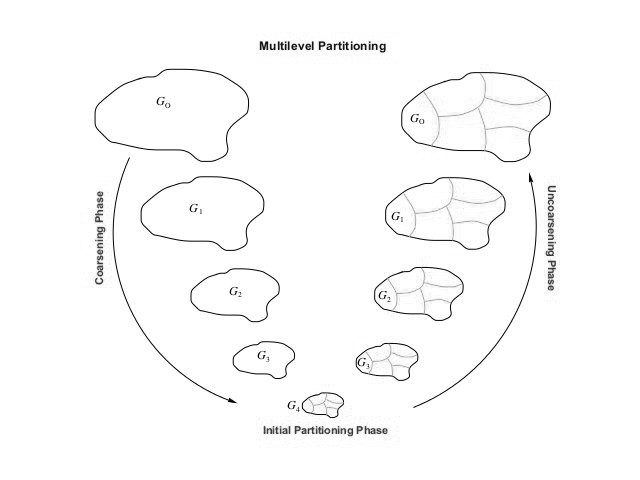
\includegraphics[scale=0.59]{Figures/metis.jpg}
	\rule{35em}{0.6pt}  % UnderLine figure	
    \caption[METIS-]{Οι τρεις φάσεις του multilevel k-way graph partitioning. Κατά την διάρκεια της συμπίεσης (coarsening), το μέγεθος του γράφου μειώνεται επιτυχώς.
    Κατά την διάρκεια του initial partitioning, υπολογίζεται ένα k-way partitioning. Κατά την διάρκεια της multilevel refinement (ή
    uncoarsening) φάσης, οι κατατμήσεις αποσυμπιέζονται διαδοχικά και προβάλλονται σε όλο και μεγαλύτερους γράφους. G0 είναι ο input γράφος, ο οποίος είναι ο λιγότερο συμπιεσμένος.
    Gi+1 είναι ο αμέσως πιο συμπιεσμένος γράφος και ο G4 είναι ο πιο συμπιεσμένος γράφος που θα υπάρξει. \cite{karypisΜetis}}
  \label{fig:metisFig}
  \end{center}
\end{figure}

    
Η ενσωμάτωση του Metis στον java κώδικα μας πραγματοποιείτε με τη χρήση της κλάσης Gpmetis \cite{GpMetis} της βιβλιοθήκης χειρισμού γράφων Grph,
η οποία αναλαμβάνει τη μεταγλώττιση (compile) του C κώδικα σε πραγματικό χρόνο, την εκτέλεση των διαδικασιών και τον χειρισμό του Ι/Ο.

 % Θεωρητική Ανάλυση

\chapter{Σχεδιασμός} % Main chapter title

\label{Σχεδιασμός} % Change X to a consecutive number; for referencing this chapter elsewhere, use \ref{ChapterX}

\lhead{Κεφάλαιο 3. \emph{Σχεδιασμός}} % Change X to a consecutive number; this is for the header on each page - perhaps a shortened title


%----------------------------------------------------------------------------------------
%	SECTION 1
%----------------------------------------------------------------------------------------


\section{socialPServer}
\noindent
Όπως προαναφέρθηκε, η προσέγγιση που ακολουθάτε στην παρούσα εργασίας αφορά την επέκταση ενός συστήματος συστάσεων ώστε να μπορεί να εξάγει συμπεράσματα για τους χρήστες του μελετώντας τον κοινωνικό τους γράφο.
Με αυτό τον τρόπο θα βελτιωθεί η ακρίβεια των συστάσεων με παραδοχή πως οι χρήστες τείνουν να έχουν κοινά ενδιαφέροντα και προτιμήσεις
με τους ανθρώπους τους οποίους έχουν επιλέξει να είναι κοινωνικά συνδεδεμένοι.
Αυτό πρακτικά σημαίνει πως έχοντας κάποιας μορφής κοινωνικό γράφο μπορούν να ομαδοποιηθούν τα μέλη του (χρήστες) σύμφωνα
με τις ακμές φιλίας ή εμπιστοσύνης που τους ενώνουν. Εντοπίζονται δηλαδή ομάδες (communities) \emph{στενά συνδεδεμένων χρηστών}
οι οποίες αποτελούν πηγή εξόρυξης διαφόρων τύπων δεδομένων. Συγκεκριμένα, πρόκειται να αξιοποιηθεί η ύπαρξη κάποιου χρήστη
σε κάποια κοινωνική ομάδα για να σκιαγραφηθούν οι προτιμήσεις του.

Το πρόγραμμα που υλοποιήθηκε για την επίτευξη των παραπάνω \setlanguage{english} \emph{(social PServer)} \setlanguage{greek} έχει τους παρακάτω \textbf{στόχους}:

\begin{description}
\item \textbf{Να αποτελέσει μια πλατφόρμα στην οποία μπορούν να ενσωματωθούν αλγόριθμοι παραγωγής κοινοτήτων χρηστών δοσμένου ενός κοινωνικού γράφου.}  \hfill \\
Επομένως πρέπει να περιλαμβάνονται όλες οι απαραίτητοι μέθοδοι για τον χειρισμό τον δεδομένων και την ολοκλήρωση της διαδικασίας διατηρώντας μια εσωτερική αυτονομία των λειτουργιών.
Αυτό επιτυγχάνεται διατηρώντας σαφή είσοδο και έξοδο της κάθε διαδικασίας και δημιουργώντας τα κατάλληλα \emph{interfaces} που θα λειτουργήσουν σαν πρότυπα-οδηγοί για την προσθήκη
νέων αλγορίθμων.
\item \textbf{Να εγκατασταθεί ένας αριθμός αλγορίθμων στο πρόγραμμα.}  \hfill \\
Ώστε να δοκιμαστεί η διαδικασία αλλά κυρίως για να αποκτήσει λειτουργικότητα. Η ενσωμάτωση αλγορίθμων στο πρόγραμμα το καθιστά πλέον όντος μια μηχανή εντοπισμού
κοινοτήτων η οποία είναι εργαλείο για ανάλυση κοινωνικών δικτύων και μπορεί να εφαρμοστεί σε πληθώρα εφαρμογών από την κοινωνιολογία, ως την στοχευμένη διαφήμιση.
\item \textbf{Να ενσωματωθεί στο υπάρχον Recomendation System PServer}  \hfill \\
Να χρησιμοποιηθεί δηλαδή το πρόγραμμά μας για να επεκτείνει την λειτουργία του PServer επιτρέποντας του να παρέχει προσωποποίηση αναλύοντας τον κοινωνικό γράφο των χρηστών του.
\end{description} 


\begin{figure}[htbp]
  \begin{center}
  %\hspace{-4.0em}    
    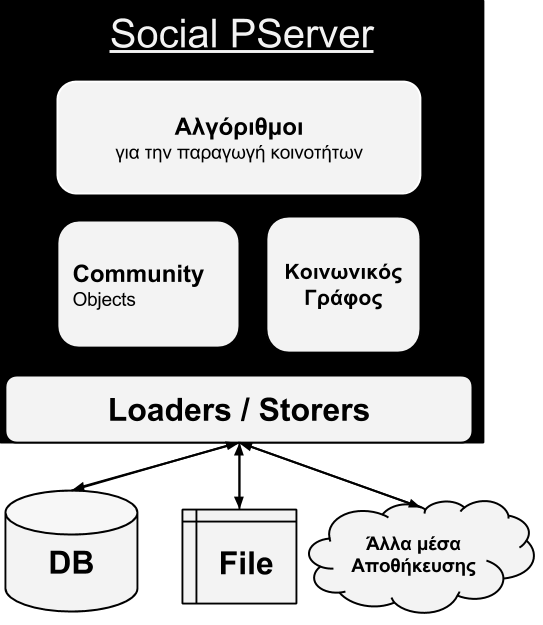
\includegraphics[scale=0.60]{Figures/socialPServerComponents.png}
	\rule{35em}{0.5pt}  % UnderLine figure	
	\caption[PServerArchitecture]{Η εσωτερική οργάνωση του socialPServer}
  \end{center}	
  \label{fig:socialPServerComponents}  
\end{figure}

\vfill

\section{Κοινωνική Πληροφορία}
\noindent
Αρχικό βήμα για την επίλυση του προβλήματος είναι να μπορούν να διαβαστούν και να επεξεργαστούν οι κοινωνικές πληροφορίες.
Το ποιες πληροφορίες πρέπει να συλλεχθούν στην την κάθε περίπτωση εξαρτάται από τη φύση αλλά και τους στόχος της υπηρεσίας.
Η συλλογή αυτών δεν αφορά τον socialPServer αλλά πραγματοποιείται από την εκάστοτε υπηρεσία. 
Κοινωνική συσχέτιση μπορεί να σημαίνει ξεκάθαρη δήλωση φιλίας από τον χρήστη άλλα μπορεί και να εντοπίζεται μέσα από την
αλληλεπίδραση του χρήστη με το σύστημα. Δηλαδή η κοινωνική πληροφορία μπορεί να εκφράζει διαφορετικά πράγματα,
αλλά αυτό που σε κάθε περίπτωση έχει ενδιαφέρον είναι η αξιοποίηση της κοινωνικής διασύνδεσης.

Η σχέση μεταξύ δυο χρηστών μπορεί να έχει διάφορες μορφές και χαρακτηριστικά. Μπορεί να είναι να έχει κατεύθυνση (directed) που σημαίνει πως κάποιος χρήστης
εμπιστεύεται κάποιον άλλον όμως μπορεί να μην συμβαίνει το αντίθετο, μπορεί να έχει κάποιο βάρος (weighted) το οποίο υποδηλώνει τον βαθμό
φιλίας των δύο ή μπορεί και να είναι undirected και unweighted να δηλώνει δηλαδή απλά την συσχέτιση δύο χρηστών. Στην τελευταία αυτή κατηγορία
έγκειται και το πρόγραμμά που υλοποιήσαμε (socialPServer) ο οποίος αποθηκεύει την εκάστοτε φιλία στην Βάση Δεδομένων καταχωρώντας μία εγγραφή τα userIDs των δύο εμπλεκόμενων χρηστών.


\subsection*{Κοινωνικός Γράφος}
\noindent
Σε αυτό το σημείο, έχοντας λοιπόν την κοινωνική πληροφορία, αρχίζει η λειτουργία του socialPServer. Το πρώτο πράγμα που πρέπει να γίνει
είναι η ανάκτηση των δεδομένων φιλίας και η δημιουργία μιας δομής δεδομένων η οποία να αντιπροσωπεύει έναν εικονικό κοινωνικό γράφο.
Για λόγους τόσο ευχρηστίας αλλά και αποδοτικότητας, για τον χειρισμό των γράφων, χρησιμοποιούνται open-source java βιβλιοθήκες στοχευμένες σε αυτό. Στη συνέχεια λοιπόν
ανάλογα με τον αλγόριθμο που θα χρησιμοποιηθεί για την παραγωγή κοινοτήτων, χρησιμοποιείται και η κατάλληλη κοινωνική δομή - γράφος.



\section{Κοινότητες χρηστών}
\noindent
Με την εφαρμογή των αλγορίθμων πρόκειται να εντοπιστούν σύνολα χρηστών τα οποία μπορούν να χαρακτηριστούν κοινότητες. Για να είναι αυτή η γνώση αξιοποιήσιμη,
σε κάθε μία από αυτές δίνεται ένα ID και στην συνέχεια για κάθε μέλος ομάδας, αποθηκεύεται στην Βάση μια εγγραφή που φέρει το UserID και το ComminityID. Με αυτόν το τρόπο μπορεί ο διαχειριστής της εκάστοτε υπηρεσίας
με μία ερώτηση στη βάση (query) να γνωρίζει ποιοι χρήστες αποτελούν ομάδα, ποιος είναι ο κοινωνικός κύκλος του κάθε χρήστη και λοιπές πληροφορίες.

\section{Προφίλ Χρήστη (userProfile)}
\noindent
Για να μπορούμε τελικός να παραχθούν συστάσεις, πρέπει εκτός από την κοινωνική πληροφορία να είναι γνωστές και οι προτιμήσεις των χρηστών, που είναι οι υπάρχουσες αξιολογήσεις αντικειμένων. 
Επομένως πρέπει να υπάρχει ένα \emph{προφίλ χρήστη} το οποίο θα περιέχει τις κάθε φορά απαραίτητες πληροφορίες 
που μας επιτρέπουν να σκιαγραφήσουμε τα ενδιαφέροντα και την συμπεριφορά του. Στην περίπτωσή μας αυτή η διαδικασία πραγματοποιείται είδη στον PServer, 
αφού πρόκειται για μια υπάρχουσα, λειτουργική και εφαρμοσμένη μηχανή προσωποποίησης. Συγκεκριμένα το \emph{user profile} περιλαμβάνει πληροφορίες για τις προτιμήσεις των χρηστών αλλά και
για τα δημογραφικά τους χαρακτηριστικά. Στα πλαίσια αυτής της εργασίας χρησιμοποιούμε τις πληροφορίες των προφίλ για να αξιολογούμε την διαδικασία παραγωγής κοινοτήτων χρησιμοποιώντας 
υπάρχοντα δεδομένα (εσωτερική αξιολόγηση). Οι προτιμήσεις των χρηστών θα ξαναχρησιμοποιηθούν όταν θα γίνουν τελικά οι συστάσεις αλλά αυτό όπως φαίνεται και από την παραπάνω περιγραφή του συστήματος, είναι 
λειτουργία του εκάστοτε recommendation engine που ανάλογα με την περίπτωση θα υπολογίσει τις πιθανές αξιολογήσεις.

\section{PServer}
\label{PServer}
\noindent
Σε αυτό το σημείο θα δοθεί περαιτέρω εξήγηση για την υπάρχουσα πλατφόρμα την οποία καλείτε να επεκτείνει το δικό μας πρόγραμμα. 
Ο PServer\cite{pServer} είναι ένας γενικής χρήσης \emph{personalization Server} οποίος είχε αναπτυχθεί από το ερευνητικό κέντρο \textbf{Δημόκριτος} και στην συνέχεια από τον οργανισμό \textbf{SciFY}.
Επόμενος πρόκειται για να λειτουργικό πρόγραμμα που μπορεί να εγκατασταθεί σε διαφορετικών ειδών εφαρμογές
για να προσφέρει προσωποποιημένη υπηρεσία. Με τον όρο προσωποποίηση εννοούμε διαφοροποίηση του περιεχομένου μιας υπηρεσίας ανάλογα με τις προτιμήσεις και την αισθητική του κάθε χρήστη.
\cite{pServerUserGuide}\\
Προσωποποίηση επιτυγχάνεται με διαφορετικούς τρόπους όπως εμφάνιση διαφορετικού GraphicalUserInterface σε κάθε χρήστη ώστε να είναι 
προσιτό σε αυτόν, προβολή διαφημίσεων που αφορούν μόνο αντικείμενα για τα οποία χρήστης έχει δείξει ενδιαφέρον στο παρελθόν και άλλους. 
Ο PServer περιλαμβάνει τις λειτουργίες που χρειάζονται για να υπάρξει ένα σύστημα συστάσεων. Αποτελεί δηλαδή την μηχανή η οποία θα αναλάβει να 
να οργανώσει τα προφίλ των χρηστών και να τους κατηγοριοποιήσει ώστε να μπορέσουν να εξαχθούν συμπεράσματα για τις προτιμήσεις τους.\\



Η λειτουργία του περιλαμβάνει τα εξής λογικά επίπεδα. 
\begin{description}
\item \textbf{Personal user models}  \hfill \\
Είναι ουσιαστικά οι πληροφορίες που αποθηκεύονται για κάθε χρήστη ώστε να μπορεί να δημιουργηθεί 
ένα user profile. Μπορεί να είναι δημογραφικά χαρακτηριστικά (\emph{Attributes} - πχ. ηλικία, φύλο) ή πληροφορίες περιεχομένου
(\emph{Features}) που αναφέρονται στην οντολογία της κάθε εφαρμογής (πχ αξιολογήσεις αντικειμένων).
\item \textbf{Stereotypes}  \hfill \\
Είναι ομάδες χρηστών με κοινά δημογραφικά χαρακτηριστικά (Attributes), οι οποίες παράγονται από τον PServer. 
\item \textbf{User Communities}  \hfill \\
Ομάδες χρηστών που προκύπτουν από την αλληλεπίδρασή τους με το σύστημα. Προς το παρόν οι χρήστες ομαδοποιούνται από 
τον PServer με βάσει τα Feature τους.
Σε αυτό το λογικό επίπεδο ανήκει και το πρόγραμμά μας, το οποίο πρόκειται να εντοπίζει τέτοιου είδους
ομάδες μελετώντας την κοινωνική συσχέτιση των χρηστών.
\end{description} 
\cite{pServerUserGuide}

\section{Αρχιτεκτονική του PServer}
\noindent
Ο PServer έχει σχεδιαστεί ώστε να είναι ανεξάρτητος από την υπηρεσία και την πλατφόρμα, με την έννοια ότι
μπορεί να λειτουργήσει σε διαφορετικά Λειτουργικά Συστήματα και μπορεί να προσφέρει υπηρεσίες προσωποποίησης 
σε κάθε εφαρμογή ανεξαρτήτως περιεχομένου. Για την επίτευξη των παραπάνω, η υλοποίησή του έχει γίνει σε java
χωρίς καθόλου χρήση API του λειτουργικού συστήματος. Το μόνο που απαιτείται είναι το μηχάνημα να διαθέτει
ένα port με Java virtual machine version 1.5+. Επίσης για να λειτουργήσει χρειάζεται μία 
σχεσιακή βάση δεδομένων, συγκεκριμένα χρησιμοποιεί MySQL 5+, η οποία είναι ανοιχτού κώδικα και 
λειτουργεί σε όλα τα διαδεδομένα Λειτουργικά Συστήματα. Τέλος για να διατηρεί ανεξαρτησία από την 
πλατφόρμα είναι σχεδιασμένος ώστε να επικοινωνεί χρησιμοποιώντας HTTP πρωτόκολλο.
Δέχεται Http requests από τις εφαρμογές που εξυπηρετεί, τα οποία περιλαμβάνουν εντολές και παραμέτρους και δίνει απάντηση σε μορφή XML ή JSON.
\cite{pServerUserGuide}

Ο PServer μπορεί να εξυπηρετεί ταυτόχρονος πολλές WEB υπηρεσίες τις οποίες ξεχωρίζει με ένα \emph{ClientID}.
Κάθε εγγραφή που αποθηκεύεται στην βάση έχει και μια στήλη με αυτό το χαρακτηριστικό ώστε να ξεχωρίζεται το περιεχόμενο των διαφορετικών πελατών του.
Σε κάθε HTTP request, εμπεριέχονται επίσης το ClientID ένας κωδικός για την αυθεντικοποίηση της υπηρεσίας.

Κάθε υπηρεσία κάνει διαφορετικές ενέργειες ώστε να προσωποποιήσει το περιεχόμενό της. 
Αυτό που προσφέρει ο PServer είναι οι απαραίτητες πληροφορίες που απαιτούνται για να υπάρξει ένα σύστημα προσωποποίησης. 
Για να μπορέσει μια υπάρχουσα υπηρεσία να εκμεταλλευτεί την λειτουργία του, 
πρέπει να υλοποιηθεί ένα ενδιάμεσο επίπεδο επικοινωνίας μεταξύ του PServer και της υπηρεσίας που ονομάζεται \textbf{Recommendation Engine},
του οποίου ο σχεδιασμός εξαρτάται κάθε φορά από τους στόχους της εφαρμογής.
Αυτό το επίπεδο αναλαμβάνει να τον τροφοδοτεί με δεδομένα, να δώσει τις σχετικές εντολές που χρειάζονται για την παραγωγή Στερεοτύπων και Κοινοτήτων 
και να ανακτήσει πληροφορίες από αυτόν. Επίσης εδώ θα προεπεξεργαστούν οι πληροφορίες που επιστρέφει ο PServer, ώστε να έχουν νόημα για την εκάστοτε υπηρεσία.


\begin{figure}[htbp]
  %\begin{center}
  \hspace{-3.5em}  
    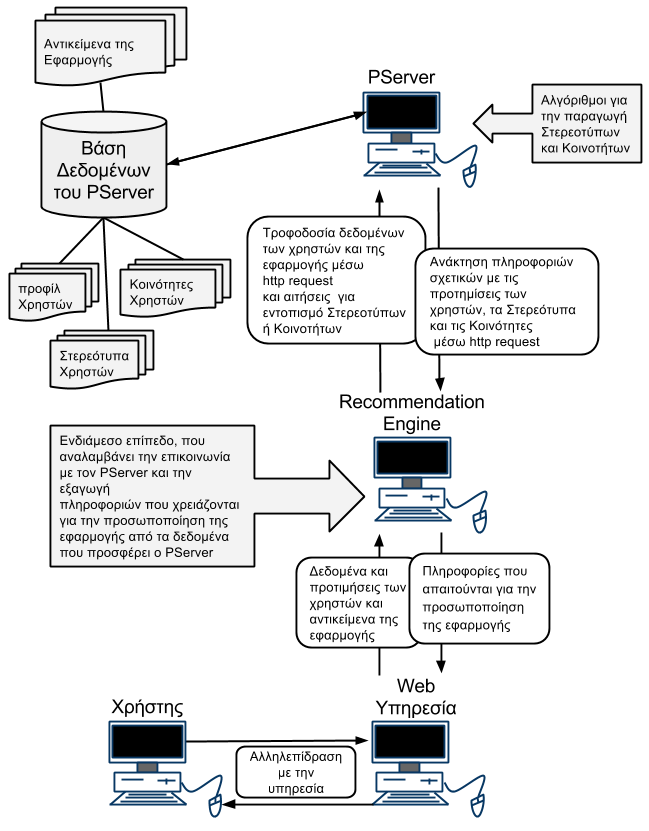
\includegraphics[scale=0.75]{Figures/PServerArchitecture.png}
	\rule{35em}{0.5pt}  % UnderLine figure	
	\caption[PServerArchitecture]{Η αρχιτεκτονική του PServer}
 % \end{center}	
  \label{fig:PServerArchitecture}  
\end{figure}


\vfill

\section{ενσωμάτωση στον PServer}

\noindent
Σημαντικός παράγοντας της αρχιτεκτονικής του προγράμματός μας είναι η αυτονομία και η μεταφερσιμότητα, ώστε να μπορεί να συμπεριληφθεί σε οποιαδήποτε άλλη java εφαρμογή σαν βιβλιοθήκη.
Έτσι και στην περίπτωση του PServer ενσωματώθηκε σαν βιβλιοθήκη και για να γίνει χρήση των λειτουργιών του καλείται με τις ανάλογες παραμέτρους που αφορούν την επιλογή του αλγορίθμου και τις
παραμέτρους αυτού.

Η λειτουργία του socialPServer απαιτεί ένα μέσο αποθήκευσης Δεδομένων στο οποίο να εμπεριέχονται τα στοιχεία των χρηστών και της εφαρμογής,
επομένως κατά την εγκατάστασή του σε κάποιο μηχάνημα ο προγραμματιστής δημιουργεί την σχετική Βάση Δεδομένων ή κάποιου τύπου αρχείο με τις απαραίτητες πληροφορίες.
Εφόσον σκοπός είναι να επεκταθούν οι υπάρχουσες λειτουργίες του PServer καλύτερο θα ήταν να χρησιμοποιεί κοινή Βάση Δεδομένων με αυτόν. 
Για να μπορούν λοιπόν να συνεργάζονται σε επίπεδο δεδομένων, στο πρόγραμμά μας χρησιμοποιούνται οι υπάρχουσες μέθοδοι που είναι υλοποιημένες στον pServer για την αλληλεπίδραση με την Βάση.
Επομένως δημιουργήσαμε ένα ενδιάμεσο επίπεδο που μεταφράζει την επικοινωνία μας με την Βάση στις μεθόδους επικοινωνίας του PServer. 
Πρακτικά λοιπόν όταν ο pServer καλεί το πρόγραμμά μας δίνει ως παράμετρο και 
ένα αντικείμενο της κλάσης του \emph{DBAccess} το οποίο περιλαμβάνει μεθόδους για τον χειρισμό των πινάκων με τους οποίους λειτουργεί.
Αυτό το αντικείμενο δίνουμε κατά την αρχικοποίηση στην δικιά μας ενδιάμεση κλάση η οποία θα αναλάβει να μεταφράζει όλες τις επικοινωνίες 
του προγράμματός μας σε επικοινωνίες του pServer.

Τέλος, στην πλευρά του PServer, προστέθηκαν κάποιες λειτουργίες στο API του χρησμού του,
ώστε να μπορεί η κάθε υπηρεσία που τον χρησιμοποιεί να τον τροφοδοτήσει με την 
απαραίτητη πληροφορία φιλίας αλλά και να χρησιμοποιεί τους Αλγορίθμους του.\\
Συγκεκριμένα ο PServer ενημερώθηκε καταλλήλως για να μπορεί να δεχτεί αιτήσεις που δηλώνουν την φιλία χρηστών και αιτήσεις
για παραγωγή κοινοτήτων χρηστών με βάση την κοινωνική πληροφορία.


\begin{figure}[htbp]
  %\begin{center}
  \hspace{-8.5em}  
    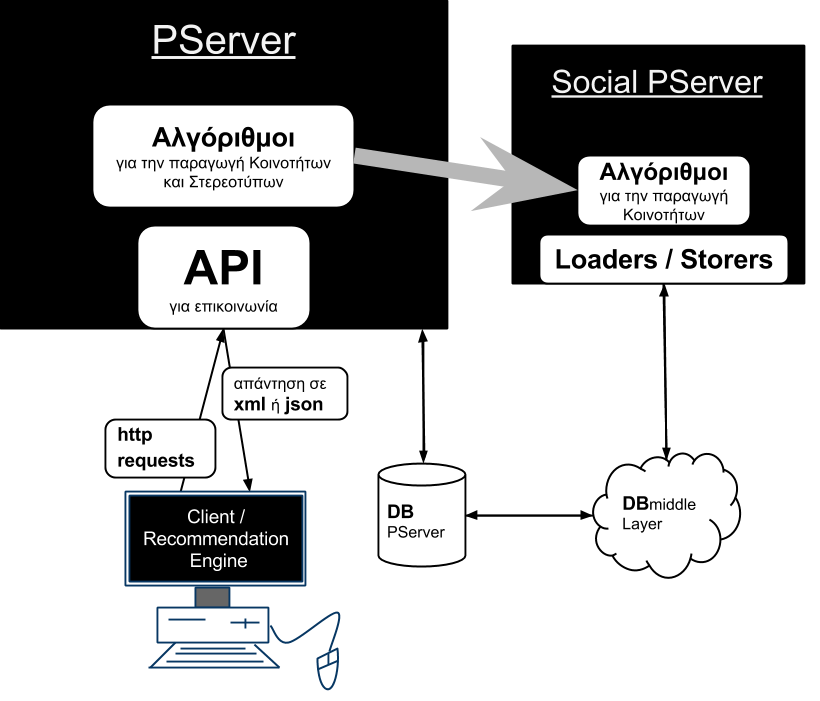
\includegraphics[scale=0.70]{Figures/socialPServer_PServer_combine.png}
	\rule{35em}{0.5pt}  % UnderLine figure	
	\caption[PServerArchitecture]{ενσωμάτωση του socialPServer στον PServer\\
	Το βέλος που ενώνει τους δυο μηχανισμούς Αλγορίθμων συμβολίζει την περίπτωση
	που ο Client, μέσω του API, ζητά τον εντοπισμό κοινοτήτων με βάση τους κοινωνικούς δεσμούς
	και επομένως\\ ο PServer καλεί τον socialPServer}
 %\end{center}	
  \label{fig:socialPServer_PServer_combine}  
\end{figure}


 % Σχεδιασμός
% Chapter Template

\chapter{Υλοποίηση} % Main chapter title

\label{Υλοποίηση} % Change X to a consecutive number; for referencing this chapter elsewhere, use \ref{ChapterX}

\lhead{Κεφάλαιο 4. \emph{Υλοποίηση}} % Change X to a consecutive number; this is for the header on each page - perhaps a shortened title
\noindent
Σε αυτό το κεφάλαιο θα γίνει μια ανασκόπηση της υλοποίησης του \setlanguage{english} socialpserver \setlanguage{greek}, θα περιγραφούν ο java κώδικας, οι διαφορετικές κλάσεις και οι μέθοδοι που αναπτύχθηκαν.
Οι κλάσεις που χρησιμοποιούνται είναι χωρισμένες στα εξής πακέτα.


\begin{description}
\item \textbf{  \hyperref[socialpserver]{ socialpserver   \ref*{socialpserver} } }  \hfill \\
Το οποίο περιλαμβάνει τις βασικότερες για την λειτουργία, κλάσεις του socialPServer.
\item \textbf{ \hyperref[socialpserver.algorithmic]{ socialpserver.algorithmic   \ref*{socialpserver.algorithmic} }  }  \hfill \\
Στο οποίο βρίσκονται κλάσεις σχετικές με τους αλγορίθμους που χρησιμοποιούνται για την παραγωγή communities.
\item \textbf{  \hyperref[socialpserver.dataio]{ socialpserver.dataio   \ref*{socialpserver.dataio} }  }   \hfill \\
Που περιλαμβάνει όλες τις κλάσεις που σχετίζονται με την είσοδο και έξοδο Δεδομένων. 
\end{description}


\section{Πακέτο socialpserver}
\label{socialpserver}
\noindent
To πακέτο αυτό περιλαμβάνει τα δομικά εργαλεία του project. Εδώ βρίσκονται οι κλάσεις που περιγράφουν τις δομές δεδομένων οι οποίες θα αντιπροσωπεύσουν τα αποτελέσματα,
δηλαδή τα communities χρηστών καθώς και η main method. Εδώ επίσης έχουν τοποθετηθεί ως υπο-πακέτα τα υπολειπόμενα πακέτα της εφαρμογής: \emph{.algorithmic} και \emph{.dataio} \\
συγκεκριμένα εμπεριέχονται οι κλάσεις:

\begin{itemize}
\renewcommand{\labelitemi}{$\star$}
\item \textbf{  \hyperref[main]{ SocialSPerver-main   \ref*{main} } } 
\item \textbf{  \hyperref[Community]{ Community   \ref*{Community} }  }  
\item \textbf{  \hyperref[SetOfCommunities]{ SetOfCommunities   \ref*{SetOfCommunities} }  } 
\end{itemize}


\begin{figure}[htbp]
  %\begin{center}
  \hspace{-3.0em}    
    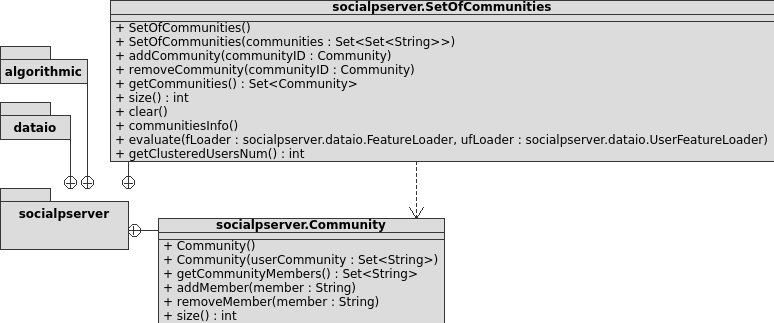
\includegraphics[scale=0.80]{Figures/socialpserverPackageClassDiagram.png}
	\rule{35em}{0.5pt}  % UnderLine figure	
	\caption[socialPServerClassDiagram]{socialPServer Package classDiagram}
  %\end{center}	
  \label{fig:socialPServerClassDiagram}  
\end{figure}


\subsection{SocialPServer-main}
\label{main}
\noindent
Εδώ βρίσκεται και η μέθοδος \textbf{main} η οποία ταξινομεί τις λειτουργίες του προγράμματος. Σε πρώτο στάδιο η main καλείται να κάνει τις απαραίτητες αρχικοποιήσεις 
επομένως δημιουργεί την αρχική σύνδεση με την Βάση Δεδομένων την οποία θα χρησιμοποιήσουν οι ακόλουθες λειτουργίες και αρχικοποιεί τους \emph{Loggers} ώστε να διαχειρίζονται
με αποδοτικό τρόπο τα μηνύματα εξόδου. Στη συνέχεια δημιουργεί τους \emph{DataLoaders} που θα αναλάβουν το πέρασμα των απαραίτητων δεδομένων και ανάλογα με την λειτουργία
που πρέπει να εκτελεστεί καλεί τους αλγορίθμους να παράξουν κοινότητες. Τέλος διαχειρίζεται την έξοδο αυτών αποθηκεύοντας την παραγόμενη πληροφορία ή καλώντας 
την αξιολόγηση των αποτελεσμάτων.

Στην βασική αυτή κλάση ακόμα περιλαμβάνεται και η μέθοδος \textbf{socialUtils} η οποία παρέχει τις αρχικές πληροφορίες για τον κοινωνικό γράφο,
πράγμα που βελτιώνει την λειτουργικότητα καθώς οι πληροφορίες αυτές είναι χρήσιμες τόσο για τον προγραμματιστή
αλλά και για τον διαχειριστή της εκάστοτε υπηρεσίας, αφού εδώ γίνονται γνωστά χαρακτηριστικά όπως το πλήθος των χρηστών και των ακμών φιλίας.


\subsection{Community}
\label{Community}
\noindent
Σε αυτό το σημείο θα περιγραφεί τι πραγματικά σημαίνει κοινότητα χρηστών (community) για τον πρόγραμμά μας.
Για να μπορεί ο socialPServer να αντιληφθεί και να χειριστεί μια κοινότητα έχει υλοποιηθεί η κλάση \textbf{Community}
η οποία είναι η Δομή Δεδομένων που αντιπροσωπεύει μια τέτοια ομάδα χρηστών.
Επομένως για κάθε παραγόμενη κοινότητα δημιουργούμε ένα νέο αντικείμενο αυτής της κλάσης και του περνάμε τις απαραίτητες πληροφορίες.

Ποιο αναλυτικά, η βάση μιας κοινότητας είναι ένα \textbf{java HashSet} που περιλαμβάνει userIDs.
Ένα java Set είναι ιδανικό για να περιγράψει μια κοινότητα αφού, θέλουμε τα μέλη να είναι μοναδικά (\emph{unique}) 
και δεν μας απασχολεί η σειρά με την οποία είναι αποθηκευμένα (\emph{unordered}).
Επίσης επιλέχθηκε συγκεκριμένα HashSet γιατί είναι η πιο αποδοτική δομή για τον χειρισμό τέτοιου είδους δεδομένων σε επίπεδο πόρων.\\
Με αυτήν την κλάση μπορούμε να προσθέσουμε τις επιπλέον λειτουργίες που χρειάζεται το πρόγραμμα καθώς και να προστατεύσουμε τη δομή από τη χρήση λειτουργιών των java Sets που
δεν χρειάζονται στην προκειμένη περίπτωση και θα ήταν εν δυνάμει καταστροφικές. Ουσιαστικά έτσι δημιουργείται ένα 'υψηλότερο' επίπεδο χειρισμού δεδομένων αφού οι διάφορες μέθοδοι
αλληλεπιδρούν με την κοινότητα μέσω αυτής της κλάσης.

Εμπεριέχεται μία global μεταβλητή:
\begin{lstlisting}[frame=single]  % Start your code-block

  private Set<String> community;
\end{lstlisting}


Αρχικά, με την δημιουργία ενός τέτοιου αντικειμένου ενεργοποιείται ο  \setlanguage{english} \textbf{constructor} \setlanguage{greek} που μπορεί να πάρει δύο μορφές, ανάλογα με το input που δίνεται.\\
Στην πρώτη περίπτωση μπορεί να δημιουργήσει κανείς ένα τέτοιο αντικείμενο χωρίς να δώσει κάποια παράμετρο
γράφοντας:

\begin{lstlisting}[frame=single]  % Start your code-block

  Community comID = new Community();
\end{lstlisting}
 
  
  όπου ο \emph{constructor} αρχικοποιεί το \emph{global community} με αυτόν τον τρόπο:
  
\begin{lstlisting}[frame=single]  % Start your code-block

  public Community() {
    this.community = new HashSet<>();
  }
\end{lstlisting}
 

  ή σε άλλη περίπτωση μπορεί από την πρώτη στιγμή να δώσει και το περιεχόμενο της δομής γράφοντας:
\begin{lstlisting}[frame=single]  % Start your code-block

  Community comID  = new Community(algorithm.out.comID);
\end{lstlisting}

 
  
  όπου ο \emph{constructor} αρχικοποιεί το \emph{global community} κάνοντας:
  
\begin{lstlisting}[frame=single]  % Start your code-block

  public Community(Set<String> userCommunity) {
        this.community = new HashSet<>();
        for (String user : userCommunity) {
            community.add(user);
        }
  }
\end{lstlisting}
  


Αφού αρχικοποιηθεί λοιπόν η δομή, ο δημιουργός του αντικειμένου πρέπει να μπορεί να εκτελέσει 'χαμηλότερου' επιπέδου λειτουργίες αλληλεπίδρασης. Υλοποιήθηκαν επομένως οι παρακάτω
μέθοδοι:


\begin{description}
\item \textbf{addMember}  \hfill \\
  πρόσθεση μέλους στην κοινότητα
\begin{lstlisting}[frame=single]  % Start your code-block

  community.add(member);
\end{lstlisting}
\item \textbf{removeMember}  \hfill \\
  αφαίρεση μέλους από την κοινότητα
\begin{lstlisting}[frame=single]  % Start your code-block

  community.remove(member);
\end{lstlisting}
\item \textbf{getCommunityMembers}   \hfill \\
  ανάκτηση μελών της κοινότητας
\begin{lstlisting}[frame=single]  % Start your code-block

  return community;
\end{lstlisting}
\item \textbf{size}   \hfill \\
  μέγεθος της κοινότητας
\begin{lstlisting}[frame=single]  % Start your code-block

  return community.size();
\end{lstlisting}
\end{description}



Τέλος, εδώ βρίσκονται κάποιες μέθοδοι που εμπλέκονται στην διαδικασία αξιολόγησης της παραγωγής κοινοτήτων δίνοντας σχετικές πληροφορίες, οι οποίες θα αναλυθούν
στο κεφάλαιο \textbf{\hyperref[eval]{Εvaluation 5.3} }.


\subsection{SetOfCommunities}
\label{SetOfCommunities}
\noindent
Ο κάθε αλγόριθμος πρόκειται να παράξει ένα σύνολο communities επομένως προκύπτει η ανάγκη δημιουργίας μιας δομής που θα
μπορεί να χειριστεί ένα τέτοιο σύνολο. Έτσι υλοποιήθηκε η κλάση \textbf{SetOfCommunities}.

Η δομή αυτή όπως προκύπτει και από το όνομά της βασίζεται σε ένα \emph{global java HashSet} που περιλαμβάνει
αντικείμενα τύπου \emph{Community}.\\
\begin{lstlisting}[frame=single]  % Start your code-block

  private Set<Community> communities;
\end{lstlisting}

Και σε αυτήν την περίπτωση η δημιουργία ενός τέτοιου αντικειμένου μπορεί να πάρει δύο μορφές, αναλόγως με την μορφή
του \emph{constructor} που θα υιοθετήσουμε. \\

  
Στην πρώτη περίπτωση μπορεί να δημιουργήσει κανείς ένα τέτοιο αντικείμενο χωρίς να δώσει κάποια παράμετρο: 


\begin{lstlisting}[frame=single]  % Start your code-block

  SetOfCommunities comSet = new SetOfCommunities();
\end{lstlisting}
 
  
  όπου ο \emph{constructor} αρχικοποιεί το \emph{global Set<Community> communities} με αυτόν τον τρόπο:
  
\begin{lstlisting}[frame=single]  % Start your code-block

  public SetOfCommunities() {
      this.communities = new HashSet<>();
  }
\end{lstlisting}
 
  ή σε κάποια άλλη μπορεί από την πρώτη στιγμή να δώσει και το περιεχόμενο της:
\begin{lstlisting}[frame=single]  % Start your code-block

  SetOfCommunities comSet = new SetOfCommunities(algorithm.out);
\end{lstlisting}

   
  όπου ο \emph{constructor} αρχικοποιεί το \emph{global Set<Community> communities} κάνοντας:
  
\begin{lstlisting}[frame=single]  % Start your code-block

    public SetOfCommunities(Set<Set<String>> communities) {
        this.communities = new HashSet<>();
        for (Set<String> community : communities) {
            this.communities.add(new Community(community));            
        }
    }
\end{lstlisting}
  
 
Όπως και προηγουμένως έτσι και σε αυτήν στην δομή μετά την αρχικοποίηση πρέπει να δίνονται στον προγραμματιστή
κάποιες βασικές λειτουργίες για τον χειρισμό αυτού του Set.
Υλοποιήθηκαν επομένως οι παρακάτω μέθοδοι:

\begin{description}
\item \textbf{addCommunity}  \hfill \\
  πρόσθεση κοινότητας στο Set
\begin{lstlisting}[frame=single] 
  communities.add(communityID);
\end{lstlisting}
\item \textbf{removeCommunity}  \hfill \\
  αφαίρεση κοινότητας από το Set
\begin{lstlisting}[frame=single]
  communities.remove(communityID);
\end{lstlisting}
\item \textbf{getCommunities}   \hfill \\
  ανάκτηση όλων των κοινοτήτων
\begin{lstlisting}[frame=single] 
  return communities;
\end{lstlisting}
\item \textbf{size}   \hfill \\
  πλήθος των κοινοτήτων
\begin{lstlisting}[frame=single]
  return communities.size();
\end{lstlisting}
\item \textbf{clear}   \hfill \\
  finalize, free memory. Διαγραφή όλων των κοινοτήτων για ελευθέρωση της μνήμης και επίσης διαγραφή των υπόλοιπων δομών που περιέχουν δεδομένα
\begin{lstlisting}[frame=single] 
    public void clear() {
        if (communities.size()>0) {
            communities.clear();
        }
        if (allCentroidFeatures.size()>0) {
            allCentroidFeatures.clear();
        }
    }
\end{lstlisting}  
\end{description}  
  
Επίσης για μία συνολική ανασκόπηση των κοινοτήτων υπάρχει η μέθοδος:  
\begin{description}  
\item \textbf{communitiesInfo}   \hfill \\
  η οποία δίνει γενικές πληροφορίες όπως:\\
  \textbf{maxCommunitySize, minCommunitySize, averageCommunitySize, κτλ}\\
  (συνήθως καλείται αμέσως πριν την διαδικασία Evaluation αλλά μπορεί να καλεστεί και οποιαδήποτε άλλη στιγμή
\end{description}


Τέλος εδώ βρίσκονται κάποιες μέθοδοι που εμπλέκονται στην διαδικασία αξιολόγησης \textbf{\hyperref[eval]{Εvaluation 5.3} }, οι οποίες θα αναλυθούν
στο σχετικό κεφάλαιο.


\section{Πακέτο socialpserver.algorithmic}
\label{socialpserver.algorithmic}
\noindent
Εδώ περιγράφονται οι κλάσεις που αφορούν τους αλγορίθμους που χρησιμοποιούνται για την παραγωγή κοινοτήτων.\\

Όπως αναφέρθηκε και στο κεφάλαιο \textbf{~\ref{Αλγόριθμοι}}  η εξαγωγή κοινοτήτων χρηστών 
μπορεί να γίνει με πολλούς διαφορετικούς τρόπους.
Χρησιμοποιήθηκε ένας αριθμός αλγορίθμων που  που έχουν χρησιμότητα για την δικιά μας περίπτωση 
οι οποίοι είναι δανεισμένοι από java βιβλιοθήκες ανοιχτού κώδικα.


\begin{figure}[htbp]
  %\begin{center}
  \hspace{-4.0em}    
    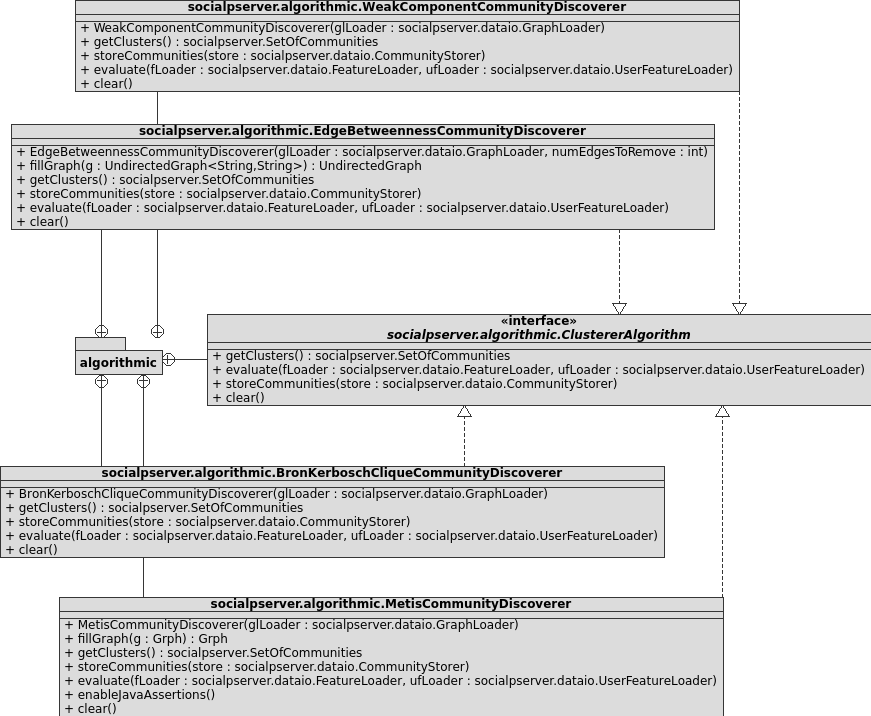
\includegraphics[scale=0.80]{Figures/algorithmicClassDiagram.png}
	\rule{35em}{0.5pt}  % UnderLine figure	
	\caption[algorithmicClassDiagram]{.algorithmic Package classDiagram}
  %\end{center}	
  \label{fig:algorithmicClassDiagram}  
\end{figure}



\subsection{interface ClustererAlgorithm}
\noindent
Αφού γίνεται χρήση αλγορίθμων που ανήκουν σε διαφορετικές βιβλιοθήκες, είναι φανερό πως πρέπει το πρόγραμμα να είναι σχεδιασμένο με τέτοιο τρόπο 
ώστε να υποστηρίζει την πρόσθεση και αφαίρεση αλγορίθμων και λειτουργιών. Πρέπει δηλαδή στην υλοποίηση να είναι ξεκάθαρα μεταξύ τους τα σημεία που είναι κοινά σε 
κάθε περίπτωση καθώς και ποιο σημείο έχει τον διαφοροποιημένο, για τον κάθε αλγόριθμο, κώδικα. 

Για λόγους λοιπόν σαφήνειας και λειτουργικότητας δημιουργήθηκε το  \setlanguage{english} \emph{interface: ClustererAlgorithm} \setlanguage{greek} το οποίο αποτελεί την σημαντικότερη κλάση στο πακέτο και 
είναι η βάση όλων των αλγορίθμων.\\
Πρόκειται για ένα πρότυπο το οποίο καθορίζει τις ελάχιστες μεθόδους που πρέπει να έχει μια κλάση του προγράμματος που αφορά αλγόριθμο.\\
Ποιο αναλυτικά:

\begin{description}
\item \textbf{imports}  \hfill \\
  καθορίζονται τα ελάχιστα imports που πρέπει να έχει μια αλγοριθμική κλάση. 
\begin{lstlisting}[frame=single] 
  import socialpserver.SetOfCommunities;    //  Data Structure
  import socialpserver.dataio.CommunityStorer;   // Data IO
  import socialpserver.dataio.FeatureLoader;   // Data IO
  import socialpserver.dataio.UserFeatureLoader;   // Data IO
\end{lstlisting}
\item \textbf{μέθοδος getClusters()}  \hfill \\
  Είναι υπεύθυνη για την εξαγωγή κοινοτήτων, θα καλεστεί τον εκάστοτε αλγόριθμο , θα δημιουργήσει το αντικείμενο SetOfCommunities, θα το επιστρέψει, κτλ     
\begin{lstlisting}[frame=single]
  public SetOfCommunities getClusters();
\end{lstlisting}
\item \textbf{μέθοδος evaluate()}   \hfill \\
  Εδώ θα καλεστούν οι μέθοδοι που χρειάζονται για αξιολογηθεί η παραγωγή κοινοτήτων και κατ επέκταση ο αλγόριθμος. (Κεφάλαιο~\ref{Αξιολόγηση})
  Επίσης συγκεκριμενοποιείται πως για να καλεστεί η μέθοδος πρέπει να δοθούν ως παράμετροι οι dataLoaders οι οποίοι θα αναλάβουν να φορτώσουν όλα τα απαραίτητα για την διαδικασία δεδομένα  
\begin{lstlisting}[frame=single]
   public void evaluate(FeatureLoader fLoader, UserFeatureLoader ufLoader);
\end{lstlisting}
\item \textbf{μέθοδος storeCommunities()}   \hfill \\
καλείται για να πραγματοποιηθεί αποθήκευση των παραγόμενων κοινοτήτων. Χρειάζεται μια παράμετρο Storer η οποία καθορίζει τον στόχο αποθήκευσης (Βάση Δεδομένων, αρχείο, κτλ).
\begin{lstlisting}[frame=single]
  public void storeCommunities(CommunityStorer store);   
\end{lstlisting}
\item \textbf{μέθοδος clear()}\hfill \\
Αναλαμβάνει να διαγράψει όσα στοιχεία δεν χρειάζονται πλέον, ώστε να ελευθερωθεί χώρος στην RAM. Συνήθως καλείται στην περίπτωση που κάποιος
για πειραματικούς λόγους θέλει να τρέχει παραπάνω από έναν αλγορίθμους με μία εκτέλεση του προγράμματος και επομένως πρέπει να ελευθερωθεί η μνήμη που χρειάστηκε
ο ένας πριν αρχίσει την διαδικασία ο επόμενος.
\begin{lstlisting}[frame=single]
  public void clear();    
\end{lstlisting}  
\end{description}

\subsection{Eνδεικτικές Yλοποιήσεις Αλγορίθμων}
\noindent
Σε αυτό το σημείο παρουσιάζονται ενδεικτικές υλοποιήσεις των παραπάνω καθώς και κάποιες ακόμα μέθοδοι, οι οποίες με ελάχιστες ή καθόλου αλλαγές έχουν νόημα για κάθε αλγόριθμο:
\begin{description}

  
\item η μέθοδος \textbf{fillGraph()}\hfill \\
Η συνάρτηση \emph{fillGraph()} φροντίζει για την δημιουργία ενός γράφου που θα περιέχει τα δεδομένα στην μορφή που τα χρειάζεται σαν είσοδο
ο κάθε αλγόριθμος. Όλες οι κλάσεις αλγορίθμων έχουν μια τέτοια μέθοδο, ο λόγος που δεν δηλώνεται στο interface είναι επειδή ο τύπος δεδομένων 
που δέχεται και επιστρέφει εξαρτάται κάθε φορά
από τον τύπου του γράφο που χρειάζεται ο εκάστοτε αλγόριθμος.

Αρχικά ενημερώνεται ο Logger για την διαδικασία που θα ακολουθήσει και ανακτάτε την πληροφορία φιλίας μέσω του Loader:
\begin{lstlisting}[frame=single]
  socialPServerOutputLogger.info("filling from given loader");                
  Set<String[]> userAssociations = loader.getGraph(); 
\end{lstlisting}   
Στη συνέχεια προσθέτονται στον γράφο οι χρήστες σαν κόμβοι και η φιλία σαν ακμή και τέλος επιστρέφεται ο γράφος.
  \begin{description}
    \item για παράδειγμα στην περίπτωση του \emph{SimpleGraph}:
\begin{lstlisting}[frame=single]
  for (String[] FriendsTable : userAssociations) {  
      g.addVertex(FriendsTable[0]);
      g.addVertex(FriendsTable[1]);
      g.addEdge(FriendsTable[0], FriendsTable[1]);
  }
  return g;
\end{lstlisting}     
  \item και στην περίπτωση του \emph{UndirectedGraph}:
\begin{lstlisting}[frame=single]
  Integer counter = 0;

  for (String[] FriendsTable : userAssociations) {
      g.addEdge(counter.toString(), FriendsTable[0], FriendsTable[1]);
      counter++;
  }
  
  return g;
\end{lstlisting}   
  \end{description}  

  
  
\item μέθοδος \textbf{getClusters()}\hfill \\
\begin{lstlisting}[frame=single]
@Override
public SetOfCommunities getClusters() {
\end{lstlisting}
Αρχικά πρέπει να δημιουργηθεί ένας κοινωνικός γράφος στην μορφή που χρειάζεται ο κάθε αλγόριθμος για να λειτουργήσει. 
  \begin{description}
    \item στην περίπτωση των\\ \emph{EdgeBetweenness} και \emph{WeakComponent}
\begin{lstlisting}[frame=single]
  UndirectedGraph<String, String> g = new UndirectedSparseGraph<>();
\end{lstlisting} 
  \item στην περίπτωση του \emph{BronKerboschClique}
\begin{lstlisting}[frame=single]
  SimpleGraph<String, DefaultEdge> g = new SimpleGraph<>(DefaultEdge.class);
\end{lstlisting} 
  \item στην περίπτωση του \emph{Metis}
\begin{lstlisting}[frame=single]
  Grph g = new Grph();
\end{lstlisting} 
  \end{description}  
Στην συνέχεια πρέπει ο γράφος αυτός να 'γεμίσει' με τους χρήστες και την πληροφορία φιλίας. Αυτό γίνεται καλώντας τη συνάρτηση \emph{fillGraph()}.
\begin{lstlisting}[frame=single]
  fillGraph(g);
\end{lstlisting} 
Πλέον ο κάθε αλγόριθμος είναι σε θέση να εντοπίσει κοινότητες χρηστών. Ενημερώνεται ο Logger για την διαδικασία που θα ακολουθήσει και καλείται η
σχετική μέθοδος: 
  \begin{description}
    \item στην περίπτωση του \emph{EdgeBetweenness}
\begin{lstlisting}[frame=single]
algorithmOutputLogger.info("trying to find communities...");        
EdgeBetweennessClusterer clusterer 
	  = new EdgeBetweennessClusterer(numEdgesToRemove);        
town = new SetOfCommunities(clusterer.transform(g));
\end{lstlisting}   
  \item στην περίπτωση του \emph{WeakComponent}
\begin{lstlisting}[frame=single]
algorithmOutputLogger.info("trying to find communities...");        
WeakComponentClusterer clusterer = new WeakComponentClusterer();        
town = new SetOfCommunities(clusterer.transform(g));
\end{lstlisting} 
  \item στην περίπτωση του \emph{BronKerboschClique}
\begin{lstlisting}[frame=single]
algorithmOutputLogger.info("trying to find communities...");                        
BronKerboschCliqueFinder bk = new BronKerboschCliqueFinder(g);
Collection cliques = bk.getAllMaximalCliques();
\end{lstlisting} 
  \item στην περίπτωση του \emph{Metis}
\begin{lstlisting}[frame=single]
algorithmOutputLogger.info("trying to find communities...");                
Gpmetis clusterer = new Gpmetis();            
List<IntSet> clusterList = clusterer.compute(g, 20, new Random(5));
\end{lstlisting} 
  \end{description}  
  Όλοι οι αλγόριθμοι δεν επιστρέφουν τις κοινότητες στην ίδια μορφή δεδομένων επομένως σε αυτό το σημείο λαμβάνουν χώρα 
  οι απαραίτητες ενέργειες για την μετατροπή των δεδομένων σε \emph{SetOfCommunities}. 
  
  
  Τέλος δίνονται στον Logger βασικές πληροφορίες για τα παραγόμενα communities (πχ πλήθος) και επιστρέφεται το παραγόμενο SetOfCommunities.
\begin{lstlisting}[frame=single]           
  socialpserver.SocialPServer.algorithmOutputLogger.info
	 ("EdgeBetweenness algoritm  ***found " + town.size() + " clusters***");                
  return town;
}   
\end{lstlisting}   

\item μέθοδος \textbf{storeCommunities()}   \hfill \\
Για την αποθήκευση κοινοτήτων έχοντας στην διάθεσή μας το αντικείμενο Storer, το οποίο απαιτείται σας παράμετρος, καλούμε την μέθοδό του .storeAll δίνοντας 
επίσης το αντικείμενο SetOfCommunities που έχει δημιουργηθεί και φορτωθεί με πληροφορία στην έξοδο του αλγορίθμου. Το μέσο της αποθήκευσης έχει καθοριστεί από αυτόν που δημιούργησε
τον Storer.
\begin{lstlisting}[frame=single]
  @Override
  public void storeCommunities(CommunityStorer store) {
      store.storeAll(socialComm);
  }
\end{lstlisting}
\item μέθοδος \textbf{clear()}\hfill \\
Η διαγραφή των εμπλεκόμενων δεδομένων γίνεται με το κάλεσμα των σχετικών μεθόδων των σχετικών δομών.
\begin{lstlisting}[frame=single]
  @Override
  public void clear() {
      socialComm.clear();
  }
\end{lstlisting}  
\item μέθοδος \textbf{evaluate()}\hfill \\
Στην αξιολόγηση αφού μελετούνται οι κοινότητες, καλούνται οι σχετικές μέθοδοι της δομής που τις αντιπροσωπεύει. 
Χρειάζεται βέβαια να τροφοδοτήσουμε με τα απαραίτητα δεδομένα, επομένως δίνουμε και ως παράμετρο τους σχετικούς dataLoaders.
\begin{lstlisting}[frame=single]
  @Override
  public void evaluate(FeatureLoader fLoader, UserFeatureLoader ufLoader) {
      town.evaluate(fLoader, ufLoader);
  }
\end{lstlisting}    
\end{description}  

\clearpage % Start a new page

\section{Πακέτο socialpserver.dataio}
\label{socialpserver.dataio}
\noindent
Σε αυτό το πακέτο βρίσκονται όλες οι κλάσεις που αφορούν την Είσοδο και Έξοδο δεδομένων στο πρόγραμμα. Συγκεκριμένα περιέχονται κλάσεις σχετικές με 
\emph{αποθήκευση δεδομένων, ανάκτηση δεδομένων,} επικοινωνία με τη \emph{Βάση Δεδομένων} και οι \emph{Loggers}.  

\vfill

\begin{figure}[htbp]
  %\begin{center}
  \hspace{-8.0em}    
    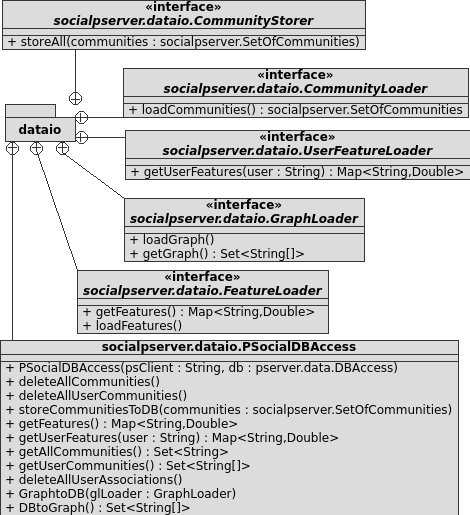
\includegraphics[scale=1.3]{Figures/dataIOClassDiagram.png}
	\rule{35em}{0.5pt}  % UnderLine figure	
	\caption[dataIOClassDiagram]{.dataIO Package classDiagram}
  %\end{center}	
  \label{fig:dataIOClassDiagram}  
\end{figure}

\clearpage

\subsection{Ανάκτηση - Αποθήκευση}
\label{Loaders - Storers}
\noindent
Για λόγους επεκτασιμότητας, στο πρόγραμμα είναι υλοποιημένα τα  \setlanguage{english} interfaces \textbf{Loaders - Storers}\setlanguage{greek}. Δίνουν στον κάθε προγραμματιστής 
την δυνατότητα να ανακτά και να αποθηκεύει δεδομένα από και σε όποιο μέσο θέλει. 
Για κάθε τύπου πληροφορία έχει υλοποιηθεί το αντίστοιχο \textbf{πρότυπο} το οποίο περιγράφει πως 
πρέπει να είναι μια κλάση χειρισμού του ανάλογου τύπου δεδομένων, 
στην οποία μπορεί να βασιστεί κάποιος και να προσθέσει τις απαραίτητες για αυτόν μεθόδους.\\

Πρότυπα:
\begin{description}
\item \textbf{CommunityStorer}   \hfill \\
  αποθηκεύει τις παραγόμενες κοινότητες, περιλαμβάνει τη μέθοδο:
\begin{lstlisting}[frame=single]
  public void storeAll(SetOfCommunities communities);
\end{lstlisting} 
\item \textbf{CommunityLoader}   \hfill \\
  ανακτά τις κοινότητες που έχουν είδη παραχθεί (χρησιμοποιείται για το Evaluation), περιλαμβάνει τη μέθοδο:
\begin{lstlisting}[frame=single]
  public SetOfCommunities loadCommunities();
\end{lstlisting} 
\item \textbf{GraphLoader}   \hfill \\
  ανακτά την πληροφορία φιλίας, περιλαμβάνει τις μεθόδους:
\begin{lstlisting}[frame=single]
  public void loadGraph();  \\ Load Graph in Memory
  public Set<String[]> getGraph();   // return Graph
\end{lstlisting} 
\item \textbf{FeatureLoader}   \hfill \\
  ανακτά όλα τα διαθέσιμα αντικείμενα της υπηρεσίας (χρησιμοποιείται για το Evaluation),
   περιλαμβάνει τις μεθόδους:
\begin{lstlisting}[frame=single]
  public Map<String, Double> getFeatures();
  public void loadFeatures();
\end{lstlisting} 
\item \textbf{UserFeatureLoader}   \hfill \\
  ανακτά τις προτιμήσεις κάθε χρήστη (αντικείμενα και αξιολογήσεις) (χρησιμοποιείται για το Evaluation), περιλαμβάνει τη μέθοδο:
\begin{lstlisting}[frame=single]
  public Map<String, Double> getUserFeatures(String user);
\end{lstlisting} 
\end{description}


\subsection*{Παράδειγμα χρήσης:}
\noindent
Για ανάκτηση της κοινωνικής πληροφορίας από την βάση Δεδομένων δημιουργούμε ένα αντικείμενο της κλάσης:\\ \setlanguage{english} \emph{GraphLoaderDB (implements GraphLoader)} \setlanguage{greek}\\
στο οποίο δίνεται ως παράμετρος ένα αντικείμενο DBAccess για να διαθέτει επικοινωνία με την Βάση.\\
Αντίστοιχα στην περίπτωση ανάκτησης του κοινωνικού γράφου από αρχείο, δημιουργούμε ένα αντικείμενο της κλάσης:\\
\setlanguage{english} \emph{GraphLoaderFile (implements GraphLoader)} \setlanguage{greek} \\
στο οποίο ως παράμετρος δίνεται η σχετική διεύθυνση του αρχείου. 
Παρόμοια διαδικασία ακολουθείται για όλες τις I/O κλάσεις.  



\subsection{DBAccess}
\label{DBAccess}

\noindent
Στην κλάση \textbf{PSocialDBAccess} είναι υλοποιημένες οι απαραίτητοι μέθοδοι για την
αλληλεπίδραση με την Βάση Δεδομένων.
Ένας από τους στόχους του socialPServer είναι η επέκταση του Pserver, 
 επομένως πρέπει να μπορεί να ανακτά και να αποθηκεύει δεδομένα που σχετίζονται 
  με τη λειτουργία του από την Βάση Δεδομένων του PServer.
Στην κλάση PSocialDBAccess βρίσκονται οι μέθοδοι που μεταφράζουν τις ανάγκες του προγράμματος για δεδομένα
  σε ερωτήσεις στην Βάση Δεδομένων του PServer.
  
Ποιο αναλυτικά, για πρόσβαση στην Βάση του PServer χρειάζεται ένα αντικείμενο \emph{pserver.data.DBAccess}.
Αυτό δίνεται ως παράμετρος στο πρόγραμμά μας και κατά την αρχικοποίηση δίνεται στην κλάση \emph{PSocialDBAccess}. 
Επίσης σαν παράμετρος δίνεται το όνομα του \emph{Πελάτη} (\emph{Client} του pServer) για τον οποίο γίνεται η διαδικασία. 
Πελάτης είναι η κάθε υπηρεσία η οποία ζητάει προσωποποίηση και πρέπει να είναι γνωστοποιημένη για να πραγματοποιηθούν επιτυχώς τα queries στη βάση,
 αφού ταυτοχρόνως ο pServer ενδέχεται να εξυπηρετεί πολλούς πελάτες. 

Κατά την υλοποίηση πρέπει να δοθεί προσοχή στις συνδέσεις που διατηρούνται 'ανοιχτές' με την Βάση γιατί μπορεί να δημιουργηθεί φόρτος στον δίαυλο επικοινωνίας.
Επομένως κατά την δημιουργία ενός αντικειμένου  \setlanguage{english} PSocialDBAccess \setlanguage{greek}:
ο Constructor αναλαμβάνει να ανοίξει και αμέσως να κλείσει μια πρώτη σύνδεση:\\\\


\begin{lstlisting}[frame=single]
  dbAccess.connect();
  dbAccess.disconnect();
\end{lstlisting}          
ώστε όλες οι μέθοδοι που θα ακολουθήσουν απλά να επανασυνδέονται:
\begin{lstlisting}[frame=single]
  dbAccess.reconnect();
\end{lstlisting}
και συνολικά το πρόγραμμα να διατηρεί μία μόνο σύνδεση με τη Βάση Δεδομένων.  


Για εγκατάσταση του socialPServer σε άλλο πρόγραμμα πρέπει να υλοποιηθεί η ανάλογη κλάση για επικοινωνία με τη Βάση (DBAccess)
  βασιζόμενη στις τωρινές μεθόδους.


\subsection{Loggers}
\label{Loggers}
\noindent
Καθ όλη την διάρκεια της λειτουργίας του, ο socialPServer δίνει μηνύματα τα οποία αποκαλύπτουν το στάδιο στο οποίο βρίσκεται η εκτέλεση,
τα βήματα που έγιναν ή ακόμα και τα λάθη που προέκυψαν.
Για την λειτουργική διαχείριση αυτών (output) χρησιμοποιούνται \emph{java Loggers} και συγκεκριμένα η default βιβλιοθήκη της java \emph{java.util.logging.Logger}.

Η διαδικασία Logging αποτελείται από τρία βασικά μέρη: \emph{Logger, Handler, Formatter}.
Έχουν υλοποιηθεί δύο σχετικές κλάσεις, η \textbf{LoggerInit} για τα πρώτα δύο και η \textbf{LoggerFormatter} για το τελευταίο.\\

Για την κάλυψη των αναγκών χρησιμοποιούνται δύο Loggers:\\
ο \textbf{socialPServerOutputLogger} ο οποίος θα αναλάβει όλο το output και το debugging του προγράμματος και ο\\
\textbf{algorithmOutputLogger} ο οποίος αφορά συγκεκριμένα την έξοδο των αλγορίθμων.

Στην κλάση \textbf{LoggerInit} η μέθοδος \textbf{initLogger} κάνει τις απαραίτητες αρχικοποιήσεις και ρυθμίσεις σχετικά με τους Loggers.
Σε πρώτο στάδιο καθορίζεται η θεμιτή \emph{ιεραρχία} των δυο Logger ώστε τα αλγοριθμικά μηνύματα να καταγράφονται αυτομάτως και στον socialPServerOutputLogger. 
\begin{lstlisting}[frame=single] 
  algorithmOutputLogger.setParent(socialPServerOutputLogger);
\end{lstlisting}

        
Στη συνέχεια καθορίζεται το \emph{output target} - \emph{Handler} που αντιπροσωπεύει το μέσω στο οποίο θα καταγράφονται τα μηνύματα. Εδώ προστέθηκαν δυο Handlers,
ένας για την εμφάνιση των μηνυμάτων στην \emph{κονσόλα} και ένας για την καταγραφή σε \emph{txt file} ώστε να είναι διαθέσιμα και μετά την εκτέλεση του προγράμματος.
\begin{lstlisting}[frame=single] 
  ConsoleHandler consoleHandler = new ConsoleHandler();
  fhAlgorithm = new FileHandler("./algorithmOutput.log");
  fhSocialPServer = new FileHandler("./socialPServerOutput.log");
\end{lstlisting}
  
Για την ομαλή λειτουργία αφού χρησιμοποιούνται καινούργιοι consoleHandlers πρέπει να απενεργοποιηθεί ο default Handler της java.
\begin{lstlisting}[frame=single] 
  LogManager.getLogManager().reset();
\end{lstlisting}

  
Επίσης καθορίζεται ποιος Handler αφορά ποιόν Logger:
\begin{lstlisting}[frame=single] 
  algorithmOutputLogger.addHandler(consoleHandler); // add consoleHandler
  algorithmOutputLogger.addHandler(fhAlgorithm);   // add FileHandler
  socialPServerOutputLogger.addHandler(fhSocialPServer);   // add FileHandler
\end{lstlisting}

 % Υλοποίηση
% Chapter Template

\chapter{Αξιολόγηση παραγόμενων κοινοτήτων} % Main chapter title

\label{Αξιολόγηση} % Change X to a consecutive number; for referencing this chapter elsewhere, use \ref{ChapterX}

\lhead{Κεφάλαιο 5. \emph{Αξιολόγηση παραγόμενων κοινοτήτων}} % Change X to a consecutive number; this is for the header on each page - perhaps a shortened title

\noindent
Εδώ περιγράφεται η προσέγγιση και οι μέθοδοι που αφορούν την αξιολόγηση των παραγόμενων κοινοτήτων (Εvaluation). 
Περιγράφονται σε ξεχωριστό κεφάλαιο αφού το Evaluation δεν αποτελεί λειτουργία του socialPServer αλλά εργαλείο του προγραμματιστή ώστε 
να μπορεί να συγκρίνει την απόδοση των αλγορίθμων.\\

Το πρόβλημα στην διαδικασίας αξιολόγησης είναι ότι δεν μπορεί να είναι ακριβής αν δεν υπάρξει ανάδραση από τους χρήστες. 
Αν δηλαδή δεν είναι γνωστό σε πιο βαθμό τα μέλη μιας κοινότητας έχουν όντως κοινά ενδιαφέροντα και προτιμήσεις.
Για να ξεπεραστεί αυτό το πρόβλημα και να υπάρχουν στοιχεία αξιολόγησης, υλοποιήθηκαν οι παρακάτω μέθοδοι στις οποίες,
έχοντας ένα DataSet που περιέχει ρεαλιστική κοινωνική πληροφορία μεταξύ των χρηστών αλλά και τις προτιμήσεις αυτών, ελέγχεται σε πιο βαθμό
υπάρχει \emph{ομοιότητα} στις αξιολογήσεις των αντικειμένων στα πλαίσια της κάθε κοινότητας.
Καθώς επίσης και σε ποιο βαθμό υπάρχει \emph{ανομοιότητα} στις αξιολογήσεις μεταξύ των διαφορετικών κοινοτήτων. 
Πρόκειται επομένως για \textbf{Εσωτερική Αξιολόγηση}.
Ακολουθεί πιο αναλυτική περιγραφή της μεθόδου καθώς και παρουσίαση των DataSet που χρησιμοποιήθηκαν.


\section{Δεδομένα (DataSets)}
\noindent
Όπως προαναφέρθηκε για να γίνει αξιολόγηση πρέπει να υπάρχουν πληροφορίες τόσο για την κοινωνική σχέση των χρηστών αλλά και για τις προτιμήσεις τους σε αντικείμενα.
Για να είναι ρεαλιστική και να έχει αποτέλεσμα η διαδικασία δεν αρκεί να δημιουργηθεί ένα ενδεικτικό σύνολο δεδομένων παράγοντας τυχαίες συνδέσεις φιλίας
και τυχαίες αξιολογήσεις αντικειμένων γιατί έτσι χάνεται το όλο νόημα της \emph{κοινωνικής πληροφορίας} η οποία εμπεριέχεται σε πραγματικούς κοινωνικούς γράφους.

Επομένως πρέπει να χρησιμοποιηθούν ρεαλιστικά δεδομένα.
Τέτοιου είδους δεδομένα σπανίζουν και συνήθως πληρώνονται αδρά, για αυτό και παρατηρείται η μανιωδώς 
συλλογή προσωπικών δεδομένων των χρηστών από τις μεγάλες εμπορικές πλατφόρμες που εμπεριέχουν κοινωνική δικτύωση.

Υπάρχουν όμως κάποια DataSets που είναι ανοιχτά για το κοινό, βοηθώντας την έρευνα, 
στα οποία είναι βασισμένες οι περισσότερες δημοσιεύσεις στον συγκεκριμένο τομέα.
Στην παρούσα εργασία εντοπίσαμε τα ακόλουθα σύνολα δεδομένων:

\begin{description}
\item \textbf{Last.FM Dataset}  \hfill \\
Πρόκειται για ένα σύνολο δεδομένων που έχει εξαχθεί χρησιμοποιώντας την υπηρεσία μουσικής προσωποποίησης Last FM\cite{LastFM} το οποίο παρουσιάστηκε κατά τη διάρκεια του 
 \setlanguage{english} 
\emph{2nd International Workshop on Information Heterogeneity and Fusion in Recommender Systems στο 5th ACM Conference on Recommender Systems}\cite{RecSys2011}.\\
 \setlanguage{greek}
Περιλαμβάνει κοινωνική δικτύωση και αξιολογήσεις καλλιτεχνών, στοιχεία που το καθιστούν ιδανικό για την δικιά μας περίπτωση.
Η έκδοση που χρησιμοποιήσαμε αποτελείται από 1892 χρήστες με 12717 ακμές φιλίας δηλαδή 25434 εγγραφές του τύπου: $undirected (user_i, user_j)$, 
όπου ο κάθε χρήστης έχει 13,443 φίλους κατά μέσο όρο.
Επίσης δίνονται 92834 αξιολογήσεις καλλιτεχνών (αντικείμενα).\\
Η συγκεκριμένη έκδοση είναι δανεισμένη από το \emph{Grouplens}\cite{grouplens}.\\
Πρόκειται για \emph{Undirected Graph}.
\item \textbf{Flixster Dataset}  \hfill \\
Δεδομένα από το Flixster.com\cite{flixster}, μια πλατφόρμα για εύρεσης ταινιών. Προσφέρει την δυνατότητα αξιολόγησης ταινιών και μπορεί να εγκατασταθεί σε κοινωνικά δίκτυα
από όπου και αντλήθηκε η πληροφορία φιλίας. Επομένως δίνει social και rating πληροφορία. 
Η έκδοση που χρησιμοποιήσαμε είναι αυτή του Mohsen Jamali\cite{MohsenJamali} η οποία περιλαμβάνει 7058820 εγγραφές φιλίας του τύπου: $undirected (user_i, user_j)$ και
8196078 αξιολογήσεις τενιών (ανικημένων).\\
Πρόκειται για \emph{Undirected Graph}.
\item \textbf{Epinions Dataset}  \hfill \\
Πρόκειται για μία διαδικτυακή υπηρεσία αξιολόγησης αντικειμένων, στην οποία κάποιος έχει την δυνατότητα να δηλώσει εμπιστοσύνη ή όχι για κάποιον άλλο χρήστη. 
Επομένως υπάρχει η πληροφορία trust-distrust η οποία συμβολίζεται με 1 ή -1 άλλα και τα ratings των αντικειμένων.\\
Αφού είναι trust και όχι social network πρόκειται για \emph{Directed Graph}. \cite{massa2006trust}
\end{description} 

Για την αξιολόγηση του socialPServer δοκιμάστηκαν δεδομένα του LastFM και του Flixster των οποίων η φύση ταιριάζει περισσότερο στην παρούσα εργασία.

\section{Σχεδιασμός της μεθόδου Αξιολόγησης}
\noindent
Μέσω της πραγματικής χρήση του προγράμματος, κάποιος θα μπορούσε να πάρει το απαραίτητο feedback για την απόδοση του συστήματος,
συλλέγοντας στατιστικά από την συμπεριφορά των χρηστών ανάλογα με τον κάθε αλγόριθμο.
Θα μπορούσε επίσης με ένα λειτουργικό σύστημα συστάσεων, να κάνει 
προτάσεις στους χρήστες και ελέγξει το τι πραγματικά είδαν.
Στο παρόν στάδιο όμως καθώς δεν έχει ολοκληρωθεί η λειτουργική ενσωμάτωση του socialPServer στον PServer, 
για να μπορεί να υπάρξει μιας μορφής αξιολόγηση και σύγκριση των αλγορίθμων 
  ακολουθείται η τυπική προσέγγιση εσωτερικής αξιολόγησης clustering που 
προτείνεται όταν στόχος είναι η ομοιότητα μεταξύ των χρηστών σε επίπεδο αντικειμένων.
Πιο συγκεκριμένα, η αξιολόγηση θεωρεί στόχο ενός "καλού" αλγορίθμου την εύρεση κοινοτήτων με 
\textbf{υψηλή intra-cluster similarity} (οι χρήστες μέσα σε μία κοινότητα είναι \emph{όμοιοι} σε επίπεδο αντικειμένων) και 
\textbf{χαμηλή inter-cluster similarity} (οι χρήστες που ανήκουν σε διαφορετικές κοινότητες είναι \emph{ανόμοιοι} σε επίπεδο αντικειμένων).
Πρόκειται για ένα κριτήριο \emph{εσωτερικής} αξιολόγησης και πρέπει να σημειωθεί πως καλή εσωτερική αξιολόγηση δεν σημαίνει απαραίτητα και καλή απόδοση του προγράμματος.\\
\cite{manning2008introduction}

Η υλοποίηση μας είναι βασισμένη στην μέθοδο αξιολόγησης \emph{Davies–Bouldin index} \cite{DaviesBouldinIndex}, η οποία παραλλάχθηκε ώστε να έχει νόημα
για την περίπτωση. 

Ποιο αναλυτικά, χρησιμοποιείται ένα μέτρο \textbf{ποιότητας συσταδοποίησης} για του οποίου τον υπολογισμό λαμβάνουν μέρος επιμέρους υπολογισμοί ομοιότητας 
(και όχι απόστασης όπως στην περίπτωση του Davies–Bouldin index).
Το μέτρο ποιότητας υπολογίζεται ως εξής:

$ Quality = \frac{Intra Simmilarity}{Inter Simmilarity}  $

όπου το Intra (Similarity) είναι η ομοιότητα που υπάρχει μεταξύ των μελών του ίδιου cluster και Inter (Similarity) η ομοιότητα που έχουν μεταξύ τους οι χρήστες διαφορετικών clusters.
Όπως είναι προφανές στόχος του κάθε αλγορίθμου είναι να έχει υψηλό Intra και χαμηλό Inter Simmilarity. 
Για αυτό και η ποιότητα υπολογίζεται με τον λόγο αυτών των δύο ώστε να τηρούνται οι
αναλογίες και να μπορούμε να συγκρίνουμε τους διαφορετικούς αλγορίθμους, με καλύτερο τον αλγόριθμο που έχει τον μεγαλύτερο λόγο (quality).
Ακολουθεί η ποιο αναλυτική περιγραφή για το πως υπολογίζονται τα μέτρα Intra και Inter Simmilarity αφού πρώτα αναφερθούμε σε κάποιες βασικές δομικές έννοιες.

\subsection{Αντιπροσωπευτικό σημείο συστάδας - centroid}
\noindent
Το πρόγραμμα μπορεί να εξυπηρετεί μεγάλο αριθμό χρηστών και τα αντικείμενα της υπηρεσίας μπορεί επίσης να είναι πάρα πολλά επομένως, η σύγκριση όλων των προφίλ χρηστών
σε μία κοινότητα μεταξύ τους θα ήταν μια δαπανηρή διαδικασία τόσο σε επίπεδο χρόνου αλλά και πόρων. 
Για αυτό υπολογίζονται και χρησιμοποιούνται κεντροϊδή σε κάθε συστάδα \textbf{Centroids}.
Για κάθε cluster δημιουργείται ένα ακόμα φανταστικό μέλος του οποίο το προφίλ (αξιολογήσεις) είναι το μέσο των αξιολογήσεων όλων των άλλων μελών. 
Αυτός ο εικονικός κόμβος είναι ουσιαστικά το κέντρο βάρους του γράφου των αντικειμένων - το σημείο που βρίσκεται στο κέντρο των αποστάσεων των προφίλ των χρηστών.
Με αυτό τον τρόπο αντί να υπολογίζεται η ομοιότητα όλων των προφίλ των χρηστών μεταξύ τους υπολογίζεται η ομοιότητα του κάθε χρήστη με τον εικονικό χρήστη Centroid.

\subsection{Μετρική ομοιότητας - cosine similarity}
\noindent
Υπάρχουν πολλές μετρικές που θα μπορούσαν να χρησιμοποιηθούν και να εκφράσουν την ομοιότητα δύο προφίλ χρηστών. 
Μία από τις πιο διαδεδομένες την οποία επιλέξαμε να χρησιμοποιήσουμε είναι η \textbf{Cosine similarity}. 
Η ομοιότητα Cosine συγκεκριμένα μετράει το συνημίτονο (cos) της γωνίας μεταξύ των δύο προφίλ.
Από την φύση της παίρνει τιμές από -1 εώς 1 αλλά στις περιπτώσεις που οι αρνητικές τιμές δεν έχουν νόημα, όπως και εδώ, παίρνει τιμές από 0 ως 1.

Ο τύπος του υπολογισμού της:

$ cosineSimilarity(A,B) = \frac{A \cdot B}{\|A\|\|B\|} = \frac{\sum\limits_{i=1}^n A_i \times B_i}{\sqrt{\sum\limits_{i=1}^n (A_i)^2} \times \sqrt{\sum\limits_{i=1}^n (B_i)^2}} $

\subsection{Μετρική ομοιότητας ζεύγους συστάδων - Intra Simmilarity}
\noindent
Ομοιότητα των μελών που βρίσκονται στο ίδιο cluster:

Έστω
\begin{description}
\item \textbf{C} το πλήθος των clusters  
\item \textbf{M} το πλήθος όλων των μελών όλων των cluster
\item \textbf{m} το πλήθος των μελών του κάθε cluster
\item \textbf{x} το κάθε Cluster
\end{description} 

βασικές έννοιες:
\begin{description}
\item \textbf{ratio(x)} cluster x size Ratio: βάρος του κάθε cluster στο συνολικό αποτέλεσμα
\item \textbf{comp(x)} cluster x Compuctness: εσωτερική ομοιότητα του κάθε cluster
\end{description} 


$ Intra = \sum\limits_{x=1}^C  comp(x) * ratio(x) $

$ ratio(x) = \frac{m_x}{M} $

\begin{description}
\item \textbf{cos(i,j)} cosine Simmilarity of memebers i - j 
\item \textbf{cent(x)} centroid of cluster x
\end{description} 


$ comp(x) = \frac{1}{m_x} * \sum\limits_{i=1}^{m_x} cos(i,cent(x)) $

Για τον υπολογισμό του \emph{Intra simmilarity} αθροίζουμε την εσωτερική ομοιότητα του κάθε cluster
πολλαπλασιασμένη με το \emph{Ratio} ώστε να επηρεάσει το τελικό αποτέλεσμα ανάλογα με το μέγεθός του.
Για να βρούμε την εσωτερική ομοιότητα του κάθε cluster (\emph{Compuctness}) αθροίζουμε την \emph{cosine simmilarity} 
του κάθε μέλους με το centroid του cluster. 

Επομένως προκύπτει:

$ InterSimmilarity = \frac{1}{M} \sum\limits_{x=1}^C \sum\limits_{i=1}^{m_x} cos(i,cent(x)) $

\subsection{Inter Simmilarity}
\noindent
Ομοιότητα των μελών που \textbf{δεν} βρίσκονται στο ίδιο cluster:

Με την ίδια λογική και σε αυτήν την περίπτωση αντί να συγκρίνουμε όλα τα μέλη των διαφορετικών κοινοτήτων
μεταξύ τους, θα συγκρίνουμε τα \emph{centroids} όλων των κοινοτήτων. 

Επομένως:

$ Inter Simmilarity = \sum\limits_{i,j=0}^C cos(cent(i),cent(j)) $

\begin{figure}[htbp]
  %\begin{center}
  \hspace{-7.5em}  
    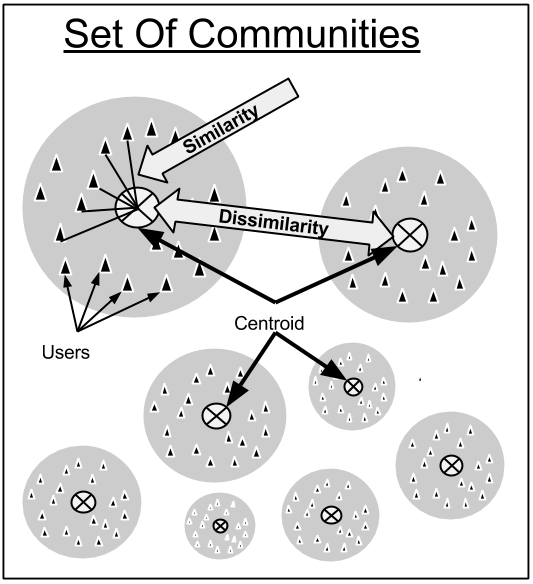
\includegraphics[scale=0.80]{Figures/evaluation_flow.png}
	\rule{35em}{0.5pt}  % UnderLine figure	
	\caption[evaluation_flow]{αξιολόγηση κοινοτήτων}
 %\end{center}	
  \label{fig:evaluation_flow}  
\end{figure}


%\vfill


\section{Υλοποίηση της Αξιολόγησης}
\label{eval}
\noindent
Οι μέθοδοι που σχετίζονται με την αξιολόγηση βρίσκονται κάθε φορά στην κλάση που αντιπροσωπεύει το αντικείμενο το οποίο θέλουμε να αξιολογήσουμε. 
Εφόσον αξιολογούνται αλγόριθμοι κάθε αλγόριθμος έχει μία μέθοδο \textbf{Evaluate}.\\
Ο κάθε αλγόριθμος περιέχει ένα αντικείμενο τύπου \textbf{SetOfCommunities} το 
οποίο αντιπροσωπεύει το σύνολο των παραγόμενων κοινοτήτων. Επομένως κάθε τέτοιου είδους αντικείμενο περιέχει επίσης μια μέθοδο \textbf{evaluation} την οποία καλεί ο εκάστοτε αλγόριθμος.
Η μέθοδος evaluation() του κάθε SetOfCommunities αναλαμβάνει να υπολογίσει το \textbf{Quality} του Set. 
Κατά την διαδικασία θα χρειαστεί να υπολογιστεί η εσωτερική ομοιότητα της κάθε κοινότητας. 
Και σε αυτήν την περίπτωση, κάθε αντικείμενο τύπου Community εμπεριέχει μια μέθοδο η οποία θα υπολογίσει το Intra Simmilarity της κάθε κοινότητας.


Κατά την διαδικασία της αξιολόγησης αρχικά υπολογίζονται κάποιες γενικές πληροφορίες για τις παραγόμενες κοινότητες όπως ο αριθμός των κοινοτήτων και το μέσο μέγεθος cluster 
και στην συνέχεια υπολογίζεται ο λόγος Quality που περιγράφτηκε παραπάνω. % Evaluation
\chapter{Εφαρμογή Προγράμματος και Αλγορίθμων Σε Πραγματικά Δεδομένα - Συμπεράσματα} % Main chapter title

\label{Εφαρμογή Σε Πραγματικά Δεδομένα - Συμπεράσματα} % Change X to a consecutive number; for referencing this chapter elsewhere, use \ref{ChapterX}

\lhead{Κεφάλαιο 6. \emph{Εφαρμογή Σε Πραγματικά Δεδομένα - Συμπεράσματα}} % Change X to a consecutive number; this is for the header on each page - perhaps a shortened title

\section{Εφαρμογή Σε Πραγματικά Δεδομένα}

\noindent Προκείμενου να αποδειχθεί πως χρησιμοποιώντας την κοινωνική πληροφορία μπορούν
να εξαχθούν συμπεράσματα για τις προτιμήσεις και την συμπεριφορά των χρηστών, δοκιμάσαμε το πρόγραμμά μας 
με δύο γνωστά DataSet. Η έρευνα είναι επιτυχής αν μέσω της μεθόδου αξιολόγησης που υλοποιήθηκε 
η μετρική \emph{Total clustering scheme compactness} είναι μεγαλύτερη από την \emph{Compactness of all centroids},
πράγμα που σημαίνει πως όντος τα μέλη μιας κοινότητας παρουσιάζουν ομοιότητες ενώ τα μέλη διαφορετικών κοινοτήτων ανομοιότητες.

$ Clusterer  Quality = \frac{Internal Simmilarity}{External Simmilarity}  $

Ο κάθε αλγόριθμος έχει άλλη προσέγγιση στον τρόπο που εντοπίζει κοινότητες 
επομένως δεν έχει νόημα η σύγκρισή τους μόνο με βάση την μετρική
\textbf{clusterer quality}.
Πρέπει να 
είναι γνωστό ένα σύνολο γενικών χαρακτηριστικών που θα αναδείξουν την συμπεριφορά του
κάθε ενός
και θα μας επιτρέψουν να επιλέξουμε τον κατάλληλο για κάθε περίπτωση χρήσης.

\clearpage

\subsection{Χαρακτηριστικά των Αλγορίθμων:} 


\begin{description}
\item \textbf{WeakComponent}  \hfill \\
Είναι στοχευμένος να εντοπίζει \emph{κλίκες}. Δηλαδή ομάδες στις οποίες όλοι οι χρήστες 
ενώνονται με όλους και αυτό τον καθιστά κατάλληλο για περιπτώσεις που είναι 
επιθυμητές κοινότητες με πυκνές συνδέσεις στο εσωτερικό.
Ομαδοποιεί μόνο όσους εμφανίζουν κλίκα και για αυτό 
μεγάλο μέρος τον χρηστών τελικά δεν ομαδοποιείται.
Λόγο της φύσης του οι κοινότητες που εντοπίζει είναι σχετικά μικρού μεγέθους 
αλλά εκτελεί την διαδικασία σε αρκετά σύντομο χρόνο διάστημα.
\item \textbf{BronKerbosch}  \hfill \\
Επίσης στοχευμένος να εντοπίζει κλίκες επομένως κοινότητες με πυκνές συνδέσεις. 
Κατάλληλος για την περίπτωσή μας αφού είναι σχεδιασμένος να εφαρμόζεται σε 
μη κατευθυνόμενους γράφους (undirected graphs) και να εντοπίζει \emph{μέγιστες κλίκες}. 
Μεγίστη κλίκα είναι ένα σύνολο χρηστών στο οποίο όλοι έχουν σύνδεση μεταξύ τους 
και δεν μπορεί να προστεθεί άλλος κόμβος στην ομάδα και να διατηρηθεί αυτή η εσωτερική 
\emph{πλήρης} συνδεσιμότητα.
To βασικό χαρακτηριστικό που τον διαφοροποιεί και τον καθιστά ευρέως 
χρησιμοποιούμενο είναι η δυνατότητά του να εντοπίζει επικαλυπτόμενες κοινότητες 
\setlanguage{english}(overlapping communities). \setlanguage{greek}Ο κάθε χρήστης μπορεί να ανήκει σε περισσότερες από 
μία κοινότητες και επομένως \emph{όλοι} οι χρήστες του γράφου ομαδοποιούνται. 
\item \textbf{EdgeBetweenness}  \hfill \\
Ιδανικός για Συστήματα Συστάσεων αφού εντοπίζει τους κεντρικούς διαύλους πληροφορίας στον γράφο.
Επίσης κατάλληλος για \setlanguage{english}Social Recommender Systems\setlanguage{greek} αφού έχει κατασκευαστεί σαν εργαλείο 
ανάλυσης κοινωνικών δικτύων που μετρά \emph{κεντρικότητα}. 
Μια ακμή έχει υψηλό \setlanguage{english}\emph{EdgeBetweenness}\setlanguage{greek} όταν βρίσκεται στα \emph{συντομότερα μονοπάτια
(Shortest Paths)} πολλών χρηστών. Αυτό την κάνει να είναι πιο "κεντρική" και επομένως
αγωγός επιρροής. Απαιτείται βέβαια χρόνος και επεξεργαστική ισχύς για τον εντοπισμό των 
shortest paths.\\

\emph{EdgeBetwenness thresshold: }Μεταβλητή που δίνεται ως παράμετρος και αντιπροσωπεύει τον αριθμό
των ακμών που θα αφαιρεθούν σταδιακά από τον γράφο. Όσες περισσότερες ακμές αφαιρούνται, τόσο μικρότερα και 
πιο πυκνά τα clusters που θα προκύψουν.

\item \textbf{Metis}  \hfill \\
Πακέτο αλγορίθμων για  την κατάτμηση γράφων οι οποίοι λειτουργούν 
κάνοντας \emph{Multilevel partitioning}. Αυτό σημαίνει πως αρχικά το μέγεθος του γράφου 
μειώνεται \emph{συμπιέζοντας (coarsening)} τους συνδεδεμένους κόμβους και ακμές. 
Στην συνέχεια ο μικρότερος πλέον γράφος κατατμείται και στην συνέχεια επαναφέρεται στο 
κανονικό του μέγεθος. Κρίθηκε κατάλληλος για την περίπτωση των κοινωνικών δικτύων 
γιατί όταν ο γράφος βρίσκεται στην πιο συμπυκνωμένη του φάση (στην οποία και κατατμείται)
έχουν συγχωνευτεί οι συνδεδεμένοι κόμβοι και επομένως αποκαλύπτονται οι διαφορετικές 
(μη συνδεδεμένες) κοινότητες.\\
Περιλαμβάνονται δύο βασικές λειτουργίες: \\
\emph{multilevel k-way partitioning (Ptype.kway)} και\\ 
\emph{multilevel recursive bisectioning (Ptype.rb)}\\
και στις δύο περιπτώσεις θα παραχθούν κοινότητες ίσου μεγέθους το πλήθος των οποίων 
δίνεται από τον χρήστη.\\
Στην περίπτωση του k-way ο γράφος χωρίζεται σε \emph{k} ίσα μέρη ενώ στην περίπτωση του 
rb πραγματοποιείται αναδρομική διαδικασία κατά την οποία ο γράφος χωρίζεται κάθε φορά
στο μισό και τερματίζει όταν υπάρξει ο επιθυμητός αριθμός κατατμήσεων. \\
Αφού οι εν λόγο αλγόριθμοι εφαρμόζονται στον συμπιεσμένο γράφο που προαναφέρθηκε
η διαδικασία πραγματοποιείται πολύ πιο γρήγορα συγκριτικά με τους παραδοσιακούς 
αλγορίθμους οι οποίοι υπολογίζουν partitions κατευθείαν στον αρχικό (μεγαλύτερο) γράφο.
\cite{miettinen}
Οι αλγόριθμοι του Metis συνίστανται σε περιπτώσεις που είναι επιθυμητή η παραγωγή κοινοτήτων 
συγκεκριμένου μεγέθους αλλά και σε περιπτώσεις γράφων μεγάλου μεγέθους.\\
Το πακέτο δίνει την δυνατότητα λεπτομερειακής παραμετροποίησης 
και με την χρήση της μεθόδου αξιολόγησης μπορεί κανείς να πραγματοποιήσει fine tuning 
στην κάθε περίπτωση χρήσης και δεδομένων.
\end{description} 

\clearpage

\textbf{Παράμετροι του Metis με την σειρά που πρέπει να δύνονται}:
%\setlanguage{english} 

%\begin{center}
\hspace{-10.5em}
    \begin{tabular}{ | p{1.7cm} | p{5.5cm} | p{12.0cm} |}
    \hline
    \emph{Παράμ.} & \emph{Χαρακτηριστικά} & \emph{Ερμηνεία} \\ \hline \hline
    \textbf{g} &   &  ο γράφος \\ \hline
    \textbf{N} &   &  αριθμός επιθυμητών κατατμήσεων \\ \hline
    \textbf{ptype} &    & καθορίζει τη μέθοδο που θα χρησιμοποιηθεί για τον υπολογισμό του
    k-way partitioning. \\ \hline
    \textbf{ctype} &    & καθορίζει τη μέθοδο που θα χρησιμοποιηθεί για να 
    να ταιριάξει τους κόμβους κατά το coarsening. \\ \hline
    \textbf{iptype} & έχει ισχύ μόνο όταν ptype=rb.  & καθορίζει τη μέθοδο που θα χρησιμοποιηθεί για
    τον υπολογισμό της αρχικής κατάτμησης του γράφου. \\ \hline
    \textbf{objtype} & έχει ισχύ μόνο όταν ptype=kway. & καθορίζει τον στόχο που οι partitioning
    routines θα βελτιστοποιήσουν. \\ \hline  
    \textbf{contig} & Αν ο γράφος δεν είναι είναι συνδεδεμένος η παράμετρος αγνοείται. Έχει ισχύ μόνο όταν ptype=kway. & Καθορίζει ότι οι partitioning routines
    θα προσπαθήσουν να παράξουν κατατμήσεις που είναι συνεχόμενες. \\ \hline
    \textbf{minconn} & έχει ισχύ μόνο όταν ptype=kway. & Καθορίζει ότι οι partitioning routines
    θα προσπαθήσουν να ελαχιστοποιήσουν τον μέγιστο βαθμό του subdomain γράφου, δηλ. του
    γράφου στον οποίο το κάθε partition είναι ένας κόμβος και οι ακμές συνδέουν τα subdomains 
    που έχουν  κοινό interface. \\ \hline  
    \textbf{ufactor} &  Για ptype=rb, προεπιλεγμένη τιμή = 1 (i.e., load imbalance of 1.001). Για ptype=kway, προεπιλεγμένη τιμή = 30 (i.e., load imbalance of 1.03). &  Καθορίζει το μέγηστο
    επιτρεπτό imbalance μεταξύ των κατατμήσεων. Μια τιμή x δηλώνει πως το επιτρεπτό load imbalance είναι $1+x/1000$. Για ptype=rb, το load imbalance μετριέται
    σαν την αναλογία: $2*max(left,right)/(left+right)$, όπου left και right είναι τα μεγέθη των αντίστοιχων partitions σε κάθε bisection (διχοτόμο γωνία). 
    Για ptype=kway, το load imbalance μετριέται σαν την αναλογία: 
    $max_i(pwgts[i])/avgpwgt$, όπου pwgts[i] είναι το βάρος του ith partition και avgpwgt είναι το άθροισμα του συνολικού βάρους των κόμβων, δια
    τον αριθμό τον ζητουμένων κατατμήσεων. \\ \hline
    \textbf{niter} & Προεπιλογή = 10. & Καθορίζει τις φορές που θα τρέξουν οι αλγόριθμοι σε
    κάθε στάδιο της διαδικασίας uncoarsening. \\ \hline  
    \textbf{ncuts} & Προεπιλογή = 1. &  Καθορίζει τον αριθμό των διαφορετικών κατατμήσεων 
    που θα υπολογιστούν. Το τελικό partition είναι αυτό που επιτυγχάνει το καλύτερο edgecut ή
    βαθμό επικοινωνίας.  \\ \hline
    \textbf{seed} &    & Διαλέγει τον "σπόρο" για την γεννήτρια τυχαίων αριθμών. \\ \hline
    \textbf{dbglvl} &    & Επιλέγει το dbglvl. \\ \hline
    \end{tabular}
%\end{center}

\clearpage


\subsection{Εφαρμογή Αλγορίθμων Ομαδοποίησης (Clustering)} 

\begin{center}
\noindent
\textbf{Χρησιμοποιώντας το Last.FM Dataset}\\
Πλήθος Χρηστών: \textbf{1892}  \hfill \\
Πλήθος κοινωνικών συνδέσεων:  \textbf{12717}  \hfill \\
\end{center}

\vspace{0.5cm}

%\begin{center}
\hspace{-10.0em}   
  \begin{tabular}{ | p{6cm} | p{3cm} | p{3cm} | l | l |}
    \hline
    \emph{Αλγόριθμος}				   & \emph{Edge Betweenness thresshold:5} & \emph{Edge Betweenness thresshold:2 } & \emph{WeakComponent} & \emph{BronKerbosch} \\ \hline \hline
    \textbf{run time}			 	   & 89.521 sec		     	   & 39.451 sec		     	    & 0.037 sec	     	    & 3.287 sec	   	\\ \hline  
    \textbf{number of Communities} 	           & 21			     	   & 20			     	    & 19		    & 11636		   \\ \hline
    \textbf{unclustered users} 	 	   & 1834		     	   & 1838		     	    & 1843   		    & 0		   	\\ \hline
    \textbf{max community size} 	 	   & 7			     	   & 7			     	    & 7  		    & 10	     	   \\ \hline
    \textbf{min community size} 	 	   & 2			     	   & 2			     	    & 2 	     	    & 2		   	\\ \hline
    \textbf{average community size}	 	   & 2.762 		     	   & 2.7 		     	    & 2.579 	     	    & 3.5090237	  	 \\ \hline
    \textbf{Total clustering scheme compactness}  & 0.5821527  	     	   & 0.5933855  	     	    & 0.6273950	     	    & 12.303899	   	\\ \hline
    \textbf{Compactness of all centroids} 	   & 0.037443716  	     	   & 0.035636988  	     	    & 0.0356979 	    & 0.13966095	   \\ \hline
    \textbf{clusterer quality} 		   & 15.547408	 	     	   & 16.650833	 	     	    & 17.575143  	    & 88.09834		   \\ 
    \hline
  \end{tabular}
%\end{center}

\vspace{1cm}

$\surd$ \noindent
Όλοι οι αλγόριθμοι παρουσιάζουν καλά αποτελέσματα σύμφωνα με την μετρική \emph{clusterer quality}
η οποία εκφράζει πως οι ομάδες χρηστών που εντοπίστηκαν παρουσιάζουν ομοιότητες περιεχομένου στο εσωτερικό
τους και ανομοιότητες σε σχέση με τις άλλες κοινότητες.
Επομένως αποδεικνύεται πως: \emph{μην έχοντας καμία πληροφορία για τις προτιμήσεις των χρηστών  
μπορούν να εντοπιστούν ομάδες χρηστών με παρόμοιες προτιμήσεις.} 

$\surd$ \noindent
Τα αποτελέσματα του BronKerbosch είναι ενισχυμένα καθώς εντοπίζει επικαλυπτόμενες κοινότητες όπου 
ο κάθε χρήστης ανήκει σε πάνω από μια ομάδες. Με αυτόν τον τρόπο παράγεται μεγάλος αριθμός
 ομάδων στενά συνδεδεμένων μελών.

$\surd$ \noindent
Στενά συνδεδεμένους χρήστες (κλίκες) επίσης εντοπίζουν οι \setlanguage{english}EdgeBetweenness και WeakComponent 
\setlanguage{greek}οι οποίοι σχηματίζουν σχετικά μικρές ομάδες (2,5-3 κόμβοι). Με το χαρακτηριστικό όμως πως 
οι χρήστες του γράφου που δεν ανήκουν σε κλίκα αγνοούνται και μένουν εκτός κοινοτήτων 
(unclustered users).

$\surd$ \noindent
Από το \emph{run time} είναι εμφανές πως ο \emph{WeakComponent} είναι ο αλγόριθμος 
που ολοκληρώνει πιο γρήγορα την διαδικασία. Ο χρόνος του \setlanguage{english}EdgeBetweenness 
\setlanguage{greek}είναι αυξημένος 
αφού χρειάζεται χρόνος για τον εντοπισμό των shortest paths. 

\vspace{11mm}

\begin{center}
\noindent
\textbf{Χρησιμοποιώντας το Flixster Dataset} \\
Πλήθος Χρηστών: \textbf{785926}  \hfill \\
Πλήθος κοινωνικών συνδέσεων: \textbf{5861294}  \hfill \\
\end{center}

\begin{center}
%\hspace{-2.0em}
  \begin{tabular}{ | p{5cm} | p{4cm} | }
    \hline
    \emph{Αλγόριθμος}				   & \emph{WeakComponent}  \\ \hline \hline
    \textbf{run time}			 	  & 17.27 sec    	    \\ \hline  
    \textbf{number of Communities} 	          & 69		\\ \hline
    \textbf{unclustered users} 	 	   & 785754 	      \\ \hline
    \textbf{max community size} 	 	  & 4 		   \\ \hline
    \textbf{min community size} 	 	      & 2 	       \\ \hline
    \textbf{average community size}	 	    & 2.4927535    \\ \hline
    \textbf{Total clustering scheme compactness}   & 0.20660953	 \\ \hline
    \textbf{Compactness of all centroids} 	     & 0.007924251	  \\ \hline
    \textbf{clusterer quality} 		    & 26.073067 	   \\ 
    \hline 
  \end{tabular}
\end{center}


\iffalse

%\begin{center}
\hspace{-5.0em}
  \begin{tabular}{ | p{3cm} | l | l | l | l |}
    \hline
    \emph{Αλγόριθμος}				   & \emph{Edge Betweenness th:5} & \emph{WeakComponent} & \emph{BronKerbosch} & \emph{Metis} \\ \hline \hline
    \textbf{run time}			 	   & sec 	     	     & 17270 sec    	     & sec		   & 108963 sec   \\ \hline  
    \textbf{number of Communities} 	           & 			     & 69		     & 			   & 9000 	   \\ \hline
    \textbf{unclustered users} 	 	   & 			     & 785754 	     	     & 			   & 0 		   \\ \hline
    \textbf{max community size} 	 	   & 			     & 4 		     & 	     		   & 89 	   \\ \hline
    \textbf{min community size} 	 	   & 			     & 2 	     	     & 			   & 0		   \\ \hline
    \textbf{average community size}	 	   &  			     & 2.4927535 	     & 	   		   & 87.32511 	   \\ \hline
    \textbf{Total clustering scheme compactness}  &   	    		     & 0.20660953	     & 			   & 0.026727572   \\ \hline
    \textbf{Compactness of all centroids} 	   &   	  		     & 0.007924251	     & 			   & 0.12443053    \\ \hline
    \textbf{clusterer quality} 		   &  	    		     & 26.073067 	     & 			   & 0.21479915    \\ 
    \hline 
  \end{tabular}
%\end{center}

\vspace{1cm}

\noindent
\textbf{EdgeBetweness thresshold: }   ti einai 

\fi


\vspace{0.5cm}

\noindent
$\surd$ Για δοκιμή του clustering στο \emph{flixster dataset} χρησιμοποιήθηκε ο 
αλγόριθμος WeakComponent ο οποίος μπορεί να παράγει αποτελέσματα σε καλό χρόνο 
σε σχέση με τους EdgeBetweenness και BronKerbosch οι οποίοι σε περιπτώσεις τέτοιας 
πολυπλοκότητας (λόγο μεγέθους) χρειάζονται πολύ χρόνο για την ανάλυση του γράφου και
την επεξεργασία των δεδομένων.


\noindent
$\surd$ Ο αλγόριθμος WeakComponent εντοπίζει κοινότητες με ομοιότητες περιεχομένου αλλά 
πολύ λίγες σε σχέσει με τον αριθμό των χρηστών. Οι περισσότεροι χρήστες μένουν εκτός 
ομάδας. Επομένως για την εξόρυξη πληροφορίας από γράφους τέτοιου μεγέθους θα χρειαστεί 
κάποιας μορφής προ επεξεργασία των δεδομένων πιθανός με χρήση αλγορίθμων partitioning
οι οποίοι θα μειώσουν την πολυπλοκότητα.

\vspace{3cm}

\clearpage

\subsection{Εφαρμογή Αλγορίθμων Κατάτμησης (Partitioning): Metis}

\vspace{1cm}

%\begin{center}
\hspace{-6.0em}   
  \begin{tabular}{ | p{4cm} | p{2.5cm} | p{2.5cm} | p{2.5cm} | p{2.5cm} |}
    \hline
    \emph{Αλγόριθμος}				   & \emph{Metis1} 	     & \emph{Metis2}	     & \emph{Metis3} 	   & \emph{Metis4}\\ \hline \hline
    \textbf{run time}			 	   & 0.221 sec 	     	     & 0.282 sec	     & 0.288 sec	   & 108.963 sec 	   \\ \hline  
    \textbf{number of Communities} 	           & 50			     & 22		     & 22		   & 9000	 	   \\ \hline
    \textbf{unclustered users} 	 	   & 0		     	     & 0   		     & 0		   & 0 		   \\ \hline
    \textbf{max community size} 	 	   & 38			     & 88  		     & 87	     	   & 89 	   \\ \hline
    \textbf{min community size} 	 	   & 35			     & 83 	     	     & 85		   & 0		   \\ \hline
    \textbf{average community size}	 	   & 37.84  		     & 86 	     	     & 86	   	   & 87.32511 	   \\ \hline
    \textbf{Total clustering scheme compactness}  & 0.26465952 	     & 0.26450196	     & 0.26567402	   & 0.026727572     \\ \hline
    \textbf{Compactness of all centroids} 	   & 0.1481018  	     & 0.18055633 	     & 0.20126359	   & 0.12443053     \\ \hline
    \textbf{clusterer quality} 		   & 1.7870108	 	     & 1.4649277  	     & 1.3200302	   & 0.21479915     \\ 
    \hline
  \end{tabular}
%\end{center}

\vspace{2cm}
\noindent
\textbf{Metis1: [Last FM]}\\ (g, 50, Gpmetis.Ptype.kway, Gpmetis.Ctype.shem, Gpmetis.Iptype.random, Gpmetis.Objtype.cut, false, false, 30, 10, 1, new Random(5)) \\
\textbf{Metis2: [Last FM]}\\ (g, 22, Gpmetis.Ptype.kway, Gpmetis.Ctype.shem, Gpmetis.Iptype.random, Gpmetis.Objtype.cut, false, false, 30, 10, 1, new Random(5)) \\  
\textbf{Metis3: [Last FM]}\\ (g, 22, Gpmetis.Ptype.rb, Gpmetis.Ctype.rm, Gpmetis.Iptype.grow, Gpmetis.Objtype.cut, false, false, 1, 10, 1, new Random(5))   \\
\textbf{Metis4: [flixster]}\\ (g, 9000, Gpmetis.Ptype.kway, Gpmetis.Ctype.shem, Gpmetis.Iptype.random, Gpmetis.Objtype.cut, false, false, 30, 10, 1, new Random(5)) 

\vspace{1cm}
\noindent
$\surd$ Τα αποτελέσματα της αξιολόγηση των αλγορίθμων partitioning δεν έχει νόημα να συγκριθούν 
με αυτά των αλγορίθμων clustering αφού έχουν διαφορετική στόχευση ως προς την επίλυση
του προβλήματος.

\noindent
$\surd$ Οι κατατμήσεις του γράφου περιλαμβάνουν μεγάλο αριθμό χρηστών και επομένως μεγάλο εύρος 
προτιμήσεων, σε αντίθεση με τους clustering αλγορίθμους που εντοπίζουν κλίκες. Για αυτό το λόγο 
και η μετρική \emph{clusterer quality} φένεται να είναι χαμηλότερη στην περίπτωση του Metis.

\noindent
$\surd$ Όλες οι κοινότητες είναι ίσου μεγέθους.

\noindent
$\surd$ Ο αριθμός των κοινοτήτων καθορίζεται από τον χρήστη.

\noindent
$\surd$ Οι δύο λειτουργίες του Metis, \emph{k-way, recursive bisectioning} στην περίπτωση
του LastFM DataSet έχουν όμοια απόδοση.

\noindent
$\surd$ Και στα δύο DataSet οι αλγόριθμοι εντοπίζουν κοινότητες χρηστών με κάποιες ομοιότητες
αλλά χωρίς να παρουσιάζονται ιδιαίτερες ανομοιότητες με τα άλλα σύνολα. Συγκεκριμένα στην
περίπτωση του flixster οι εξωτερικές ομοιότητες φαίνεται να είναι περισσότερες από τις
εσωτερικές. Αυτό δείχνει πως μόνο με την εφαρμογή του Metis μια φορά, το πρόγραμμά δεν 
είναι σε θέση να  χωρίσει τον γράφο σε κοινότητες περιεχομένου. 

\noindent
$\surd$ Ο Metis πραγματοποιεί την διαδικασία σε καλό χρόνο ακόμα 
και στο \emph{flixster DataSet}, αναλογικά με το μέγεθός του,
λόγο του ότι πρόκειται για \emph{multilevel partioner}.


\clearpage

\section{Συμπεράσματα}
\noindent
Στα πλαίσια αυτής της εργασίας πραγματοποιήθηκε μελέτη σχετικά με τα Συστήματα Συστάσεων και τον συνδυασμό τους με τα Κοινωνικά Δίκτυα.
Διερευνήθηκε ο τρόπος με τον οποίο ένα τέτοιο σύστημα μπορεί να βελτιώσει την λειτουργία του, εξάγοντας γνώση από την κοινωνική διασύνδεση των χρηστών. 
Στην συνέχεια βάση αυτής της ανάλυσης αναπτύχθηκε ένα σύστημα εξαγωγής γνώσης από κοινωνικό γράφο, με τον κατάλληλο σχεδιασμό ώστε να αποτελέσει επέκταση ενός υπάρχοντος 
Recommendation System. Πρόκειται για τον PServer, ένα γενικευμένο σύστημα Προσωποποίησης το οποίο διαθέτει μηχανισμούς συστάσεων που ακολουθούν Content Based αλλά και Collaborative μεθόδους. 
Το σύστημά μας (socialPServer) πρόκειται για έναν μηχανισμό ο οποίος είναι σε θέση να χειρίζεται έναν κοινωνικό γάφο και να εφαρμόζει έναν αριθμό αλγορίθμων εντοπισμού κοινοτήτων χρηστών. 
Οι αλγόριθμοι μελετούν τις κοινωνικές συνδέσεις με διάφορους τρόπους και συμπεραίνουν "κλίκες" στενά συνδεδεμένων χρηστών. Αυτή την κοινωνική πληροφορία πρόκειται να χρησιμοποιήσει
ο PServer για να βελτιώσει την ακρίβεια των αποτελεσμάτων του.
Σε μια ρεαλιστική κοινότητα τα μέλη μοιράζονται κοινά "αντικείμενα", για παράδειγμα κοινά συγγράμματα σε 
μία ακαδημαϊκή κοινότητα ή και κοινές αισθητικές προτιμήσεις σε έναν ευρύτερο φιλικό κύκλο. Επομένως για να επιτευχθεί η προσωποποίηση θα γίνουν υποθέσεις για τις προτιμήσεις των χρηστών 
ανάλογα με το κοινωνικό τους περιβάλλον. 

Τέλος έγινε δοκιμή του προγράμματος σε πραγματικά δεδομένα με χρίση των DataSet: LastFM και Flixster. Για να αξιολογηθούν τα αποτελέσματα χρησιμοποιήθηκαν μέτρα ομοιότητας τα οποία 
υπολογίζουν κατά πόσον μοιάζουν τα προφίλ των χρηστών, δηλαδή σε ποιο βαθμό οι υπάρχουν κοινές προτιμήσεις αντικείμενων. Σε όλες τις περιπτώσεις των αλγορίθμων οι παραγόμενες κοινότητες 
εμφανίζουν ομοιότητα στα μέλη τις ίδιας κοινότητας και ανομοιότητα στα μέλη άλλων κοινοτήτων. Το γεγονός ότι μη ξέροντας τίποτα για τις προτιμήσεις μπορούν να εντοπιστούν σύνολα χρηστών
τα οποία παρουσιάζουν ομοιότητες αποδεικνύει την δύναμη των πληροφοριών που κρύβει η κοινωνική δομή και το ενδιαφέρον για την ανάλυση των κοινωνικών δικτύων συνεχώς αυξάνεται.
 % Συμπεράσματα

\chapter{Μελλοντικές Επεκτάσεις - Προσωπικά Δεδομένα - Άδειες} % Main chapter title

\label{Μελοντικές Επεκτάσεις - Προσωπικά Δεδομένα - Άδειες} % Change X to a consecutive number; for referencing this chapter elsewhere, use \ref{ChapterX}

\lhead{Κεφάλαιο 6. \emph{Μελλοντικές Επεκτάσεις - Προσωπικά Δεδομένα - Άδειες}} % Change X to a consecutive number; this is for the header on each page - perhaps a shortened title

\section{Μελλοντικές Επεκτάσεις}

\begin{description}
\item \textbf{Βελτιστοποίηση των συστάσεων}  \hfill \\
Στο κεφάλαιο 2 (Σχεδιασμός) όπου περιγράφεται η αρχιτεκτονική του PServer γίνεται λόγος για το \emph{Recommendation Engine}, το ενδιάμεσο επίπεδο μεταξύ αυτού και της εφαρμογής. 
Σε αυτό το στάδιο επεξεργάζονται οι πληροφορίες που δίνει ο PServer ώστε να έχουν νόημα για την εκάστοτε υπηρεσία. 
Είδη έχει ξεκινήσει ο σχεδιασμός ενός τέτοιου μηχανισμού ο οποίος θα μπορεί να εκμεταλλευτεί πλήρως τις δυνατότητες του PServer συνδυάζοντας τις πληροφορίες που δίνονται σε κάθε λογικό
επίπεδό (Personal, Community, Social).
\item \textbf{Χρήση σε άλλες επιστήμες}  \hfill \\
Εμπνευσμένοι από το \emph{Community structure in jazz}\cite{jazz} όπου με \setlanguage{english} collaborative \setlanguage{greek} προσέγγιση από τις πληροφορίες για συνδέσεις των jazz μουσικών και σχημάτων προκύπτουν κοινοτικές
δομές, θα θέλαμε το πρόγραμμά μας να συμβάλει σε κοινωνικές και ανθρωπιστικές επιστήμες. Η χρήση του μπορεί να αναδείξει νέες κοινωνικές ομάδες και ρεύματα, συνεπώς μπορεί να συμβάλει
στην καλύτερη κατανόηση του κοινωνικού μας περιβάλλοντος και κατ επέκταση στην καλύτερη διαχείριση.
\item \textbf{Επικαλυπτόμενες Κοινότητες}  \hfill \\
Μελετώντας την σχετική βιβλιογραφία, η πιο πλούσια και ρεαλιστική προσέγγιση όσον αφορά τις κοινότητες συνδεδεμένων μελών που εγείρει το ενδιαφέρον μας και ανοίγει νέους ορίζοντες για έρευνα 
είναι το άρθρο \emph{Uncovering the overlapping community structure of complex networks in nature and society}\cite{overlapping}.
Οι συγγραφείς του ερμηνεύουν τα δικτυακά συστήματα στη φύση και την κοινωνία ως την συνύπαρξη των μικρότερων κοινοτήτων που τις αποτελούν. 
Αναγνωρίζοντας πως τέτοια σύνολα εμφανίζουν επικαλυπτόμενες κοινοτικές δομές, εισάγουν μετρικές και μεθόδους για την περαιτέρω μελέτη τους, προσπαθώντας να αποκαλύψουν την πραγματική τους φύση
και ξεπερνώντας τις μέχρι τώρα ντετερμινιστικές μεθόδους.
Μακροπρόθεσμος στόχος μας είναι να επεκταθεί η παρούσα εργασία σε ένα σύστημα που θα εκμεταλλεύεται τις πληροφορίες που αντλούνται από ένα περίπλοκο σύστημα με επικαλυπτόμενες
κοινότητες ώστε να εξάγει γνώσει από αυτό.
\end{description} 


\section{Προσωπικά Δεδομένα}
\noindent
Οι τεχνολογίες προσωποποίησης χρησιμοποιούνται πλέον σε πληθώρα διαδικτυακών εφαρμογών
και υπηρεσιών. Αποτελούν ανεκτίμητο εργαλείο αλλά ταυτόχρονα φέρνουν
σημαντικές δεοντολογικές συγκρούσεις στον επιστημονικό κόσμο. 
Αυτό συμβαίνει διότι κατά την δημιουργία των προφίλ χρηστών που προαναφέρθηκαν,
θίγονται ευαίσθητα θέματα και εμφανίζονται ηθικά διλήμματα τα οποία σχετίζονται με την 
\textbf{παραβίαση προσωπικών δεδομένων}.
Η διαδικασία συλλογής των δεδομένων μπορεί να πραγματοποιείται \emph{άμεσα}, 
όπως στις περιπτώσεις που ο ίδιος ο χρήστης καταχωρεί στοιχεία για αυτόν, 
είτε \emph{έμμεσα} όπως στις περιπτώσεις που βγαίνουν συμπεράσματα από την 
αλληλεπίδρασή του με το σύστημα.\cite{eirinaki2003web}\\
Και στις δυο περιπτώσεις ο χρήστης χάνει την ανωνυμία του και επομένως πρέπει να γνωρίζει πως τα προσωπικά
του δεδομένα καταγράφονται και χρησιμοποιούνται από την υπηρεσία.
Ακόμα και στις περιπτώσεις που ο ίδιος έχει επιτρέψει στην υπηρεσία την καταγραφή δεδομένων,
μέσω της χρήσης Cookies, τέτοιου είδους πληροφορίες μπορούν να ανακατευθυνθούν σε 
άλλους διαδικτυακούς τόπους ώστε να υποκλαπούν.

Σε κάθε περίπτωση εφαρμογής τέτοιου είδους τεχνολογιών πρέπει από την αρχή να γίνεται
σαφές στον χρήστη πως οι κινήσεις του καταγράφονται ώστε να φροντίζει μόνος του για την 
επιλογή των δεδομένων που θα γνωστοποιηθούν. Αυτό βέβαια προϋποθέτει πως και τα άτομα που 
διευθύνουν την υπηρεσία είναι άξια εμπιστοσύνης. Ελπίζουμε και επιδιώκουμε τα αποτελέσματα
αυτής της εργασίας να μην χρησιμοποιηθούν με αρνητική σκοπιμότητα άλλα για να 
επηρεάσουν θετικά την ανθρώπινη και την κοινωνική ζωή.

\section{Άδειες}
\noindent Στα πλαίσια της παρούσας πτυχιακής χρησιμοποιήθηκαν τα παρακάτω εργαλεία κατασκευασμένα από 
άλλους προγραμματιστές τα οποία έχουν εκδοθεί κάτω από άδειες ανοιχτού κώδικά.\\



%\begin{center}
\hspace{-9.0em}
    \begin{tabular}{ | p{4cm} | p{6cm} | p{8cm} | }
    \hline
    \textbf{project} & \textbf{Licence} & \textbf{Source} \\ \hline 
    WeakComponent & BSD open-source license & JUNG Software Library \url{http://jung.sourceforge.net/license.txt} \\ \hline  
    EdgeBetweenness & BSD open-source license & JUNG Software Library \url{http://jung.sourceforge.net/license.txt}  \\ \hline
    BronKerbosch & EPL (Eclipse) and LGPL  & jgrapht Java graph Library \url{https://github.com/jgrapht/jgrapht/wiki/Relicensing} \\ \hline
    Metis & Apache License, Version 2.0 & Karypis George \url{https://www.apache.org/licenses/LICENSE-2.0} \\ \hline  
    GPmetis & LGPL Version 3 & Grph - graph library \url{http://www.i3s.unice.fr/~hogie/grph/?page=License} \\ \hline
    betweenness figure \ref{fig:GraphBetweenness} & GNU 1.2, CC 3.0, CC 2.5 & Claudio Rocchini(2007) - Wiki \url{https://en.wikipedia.org/wiki/File:Graph_betweenness.svg} \\ \hline
    PServer & Apache License, Version 2.0 & Dimokritos - SciFy \url{http://pserver-project.org/en/content/pservers-source-code} \\ \hline
    \end{tabular}
%\end{center} % other  


\backmatter

%----------------------------------------------------------------------------------------
%	BIBLIOGRAPHY
%----------------------------------------------------------------------------------------

\label{Bibliography}

\lhead{\emph{Bibliography}} % Change the page header to say "Bibliography"

\bibliographystyle{unsrtnat} % Use the "unsrtnat" BibTeX style for formatting the Bibliography

\bibliography{Bibliography} % The references (bibliography) information are stored in the file named "Bibliography.bib"

\end{document}  


